% Greeks Engine: project report
% Compile with pdflatex (twice, for the contents and references), or upload this
% folder (with figures/) to Overleaf. Every number below comes from the
% repository: validation/results/*.csv, validation/figures/tables.md, the Vivado
% reports in validation/results/vivado/, and the ZedBoard logs.
\documentclass[11pt,a4paper]{article}

\usepackage[T1]{fontenc}
\usepackage[utf8]{inputenc}
\usepackage{lmodern}
\usepackage[a4paper,margin=2.2cm]{geometry}
\usepackage{graphicx}
\usepackage{booktabs}
\usepackage{tabularx}
\usepackage{array}
\usepackage{multirow}
\usepackage{xcolor}
\usepackage{colortbl}
\usepackage{float}
\usepackage{caption}
\usepackage{enumitem}
\usepackage{amsmath}
\usepackage{tikz}
\usetikzlibrary{arrows.meta,positioning,fit,calc,backgrounds,shapes.geometric}
\usepackage[colorlinks=true,linkcolor=accent,citecolor=accent,urlcolor=accent]{hyperref}

\definecolor{accent}{HTML}{0F6B5C}
\definecolor{accentsoft}{HTML}{DCEFE9}
\definecolor{aad}{HTML}{1FA97A}
\definecolor{bump}{HTML}{E8683A}
\definecolor{ink}{HTML}{16202A}
\definecolor{muted}{HTML}{56626B}
\definecolor{rulec}{HTML}{D5DBD3}
\definecolor{plan}{HTML}{7C9CBC}
\definecolor{hostc}{HTML}{EEF1EC}

\captionsetup{font=small,labelfont=bf,margin=0.5cm}
\setlist{itemsep=2pt,topsep=4pt}
\setlength{\parskip}{4pt}
\renewcommand{\arraystretch}{1.18}
\newcolumntype{Y}{>{\raggedright\arraybackslash}X}
\newcolumntype{R}{>{\raggedleft\arraybackslash}X}

% "why it is useful / what is new" boxes after each result
\newcommand{\useful}[1]{\par\noindent\textbf{\textcolor{accent}{Why it is useful.}} #1\par}
\newcommand{\novel}[1]{\par\noindent\textbf{\textcolor{accent}{What is new.}} #1\par}
\newcommand{\rupee}{Rs\,}
\newcommand{\hi}{\rowcolor{accentsoft}}

\tikzset{
  blk/.style={draw=accent, fill=white, rounded corners=2pt, align=center, font=\small,
              minimum height=1.0cm, inner sep=4pt},
  key/.style={blk, fill=accentsoft, font=\small\bfseries},
  hostb/.style={blk, fill=hostc, draw=muted},
  arr/.style={-{Stealth[length=2.2mm]}, thick, draw=ink},
  darr/.style={-{Stealth[length=2.2mm]}, thick, draw=muted, dashed},
  lbl/.style={font=\footnotesize, text=muted, align=center},
}

\title{\vspace{-1cm}\textbf{Option Greeks in One Hardware Pass}\\[4pt]
\large An FPGA Engine for Heston-Model Greeks by Adjoint Differentiation}
\author{Yash Agrawal\\[2pt]
\small Birla Institute of Technology and Science, Pilani\\[8pt]
\small Course registered under: \textbf{Prof.\ Natasha Hazarika}\\
\small Supervisor: \textbf{Prof.\ Govind Prasad}}
\date{\small Project report, 6 October 2026}

\begin{document}
\maketitle

% =====================================================================
\begin{abstract}
\noindent
Risk management needs not only option prices but their sensitivities to every
input, the Greeks. Under the Heston stochastic-volatility model the price has no
closed form, and the standard way to obtain Greeks, bump-and-reprice, costs 19
pricings for nine Greeks. This project builds adjoint (reverse-mode)
differentiation as a hardware datapath. The Heston price, computed by the COS
Fourier-cosine method, and its adjoint are written once as an operation graph; a
generator turns it into a fixed-point, resource-shared, modulo-scheduled Verilog
engine, together with a bit-accurate model and a first-order bound on the rounding
error of every output. The engine returns the price and all nine Greeks in 4,733 clock cycles,
only 1.04 times the cost of the price alone and 18.4 times fewer cycles than
bump-and-reprice on the same hardware. It fits a Zynq-7020 FPGA; with setup and finish
on the host, its loop takes 65.3\,$\mu$s per evaluation on a ZedBoard and produced
results bit-identical to the model on 50 random cases in silicon. Hand-derived
analytic Greeks on one laptop CPU core are faster (about 29\,$\mu$s); the engine's
gains are the cost of its Greeks and a rounding-error bound on each. Forward-mode
datapaths built by the same generator need more multipliers for the same Greeks: 25\%
more when hand-factored like analytic Greeks, 3.2 times more as an AD tool would
build them. A small case study on a year of real NIFTY option data illustrates the
Greeks in use for hedging.
\end{abstract}

\tableofcontents
\newpage

% =====================================================================
\section{Introduction}

\subsection{The problem}
A bank holding options must know, continuously, how each price responds to the
spot price, strike, maturity, interest rate and every parameter of its pricing
model. These first derivatives, the \emph{Greeks}, drive hedging and risk limits.
The Heston model~\cite{heston} lets volatility follow its own random process, which
reproduces the volatility smile that constant-volatility models cannot. Its price has
no closed form and is computed numerically; this project uses the COS
method~\cite{fang}, which expands the payoff in a 128-term cosine series and needs
only the model's characteristic function.

Two ways exist to obtain Greeks from such a pricer:
\begin{itemize}
  \item \textbf{Bump-and-reprice} nudges each input and prices again. Nine Greeks
  by central differences cost 19 pricings, and the result depends on a bump size
  with no safe choice: too small and rounding dominates, too large and truncation
  does.
  \item \textbf{Adjoint differentiation} (reverse mode, often called AAD in
  finance~\cite{giles,capriotti}) obtains every Greek from one backward sweep over
  the pricing computation, exactly and at a small constant multiple of one pricing.
  In software it records a tape of every operation and replays it backwards, which
  costs 3--7 pricings in practice~\cite{savine}.
\end{itemize}
Adjoint differentiation is standard in software. On FPGAs, every published Greeks
engine still re-runs the pricer once per sensitivity~\cite{klai1,vitis}.

Three separate layers are involved, and the project uses all three: the
\textbf{Heston model} describes how the stock and its volatility move; the
\textbf{COS method} computes the option price from that model; the \textbf{adjoint
method} computes the Greeks by differentiating the COS computation. The Greeks are
computed exactly from the model, not predicted.

\subsection{What this project does}
The Heston-COS price and its adjoint sweep are written once as an operation graph.
A generator, written for this project, produces from that single description:
\begin{itemize}
  \item a bit-accurate fixed-point model of the hardware (the golden reference);
  \item a double-precision model of the same algorithm;
  \item a first-order bound on the rounding error of the price and each Greek (the
  COS method's own truncation error is a separate term, reported in
  Section~\ref{sec:methoderr});
  \item a modulo-scheduled Verilog datapath that shares a small number of
  multipliers and CORDIC units across all operations.
\end{itemize}
The engine was implemented with Vivado on a Zynq-7020, run on a ZedBoard, and
compared against bump-and-reprice on the same hardware and against software on a
laptop CPU.

\subsection{Novelty}
\begin{enumerate}[label=\textbf{\arabic*.}]
  \item \textbf{The first FPGA implementation of adjoint (reverse-mode)
  differentiation for option Greeks.} No published FPGA Greeks engine uses
  adjoints~\cite{klai1,klai2,vitis}: the AMD library re-runs the pricer once per
  sensitivity; the 2024 survey of 99
  FPGA option-pricing studies~\cite{survey} and the 2024 review of fifteen years of
  adjoint differentiation in finance~\cite{aadreview} contain no FPGA adjoint
  implementation.
  \item \textbf{The first FPGA implementation of the COS method.} COS pricing had
  run on CPUs and GPUs~\cite{zhang}; the only FPGA Fourier pricer~\cite{vitis} uses
  trapezoidal integration and returns the price alone.
  \item \textbf{A tape-free adjoint datapath.} The reverse sweep is compiled into a
  statically scheduled fixed-point datapath that shares its arithmetic units with the
  forward pass: no tape memory and no replay logic. This is possible because the COS
  pricer performs the same operations for every input.
  \item \textbf{All nine Greeks for 1.04 times the cost of one price.} On the same
  hardware the price alone takes 4,568 cycles and the price with all nine Greeks
  4,733. On the measured CPU, Greeks derived by hand cost 1.9 pricings, AD tools
  5.3--6.7, and bump-and-reprice 19.
  \item \textbf{A first-order rounding-error bound for every Greek of a fixed-point
  adjoint datapath.} Measured error never exceeds 0.103 of the bound over 21 test cases, 0.378
  over 10,500 inputs including hard regimes, and the bound held on silicon.
  \item \textbf{Bit-exact Greeks on silicon.} On a ZedBoard (Zynq-7020), 450 of 450
  results from 50 random cases matched the model bit for bit.
\end{enumerate}

\paragraph{Prior work these points rest on.} The novelty lies in the combination
and its realisation in hardware. Reverse-mode differentiation itself is
established~\cite{linnainmaa,giles}; the error bound applies first-order rounding
analysis~\cite{linnainmaa} to a datapath that itself performs the adjoint; the
arithmetic (Newton-Raphson reciprocals, Tang's exponential, CORDIC) is standard. The
literature check behind the novelty points was made on 29 September 2026 and is
recorded in the repository (\texttt{docs/novelty\_assessment.md}).

% =====================================================================
\section{System architecture}

\subsection{Design flow}
Figure~\ref{fig:flow} shows how one description becomes every artifact. Because the
RTL and the golden model come from the same graph, the testbench checks every
register at the cycle it becomes valid (1,213 to 1,962 checks per design), not just
the outputs, and any property shown for the model holds for the hardware.

\begin{figure}[H]
\centering
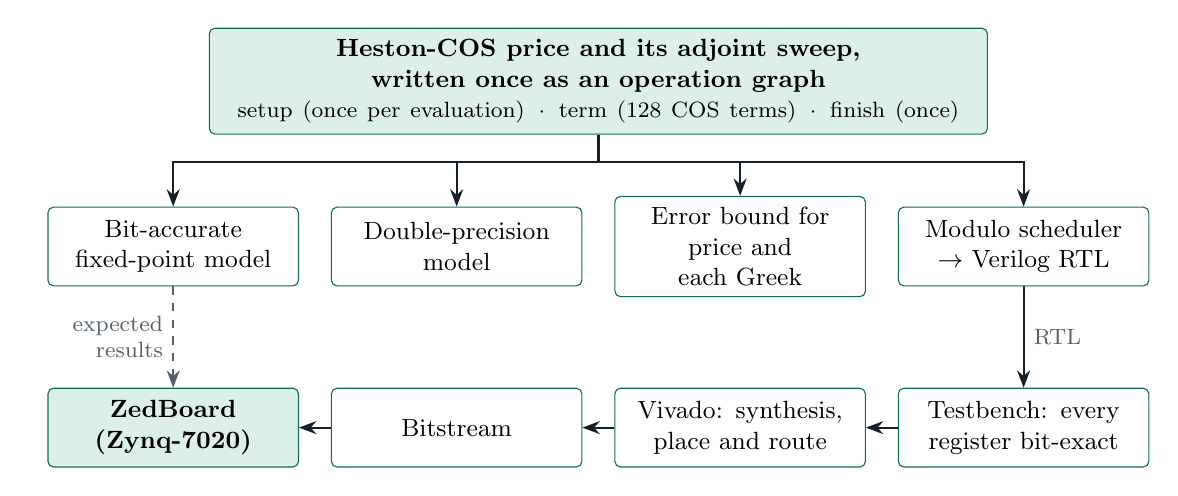
\begin{tikzpicture}
  \node[key, text width=9.6cm] (src) at (0,0) {Heston-COS price and its adjoint sweep, written once as an operation graph\\
    \normalfont\footnotesize setup (once per evaluation) \,$\cdot$\, term (128 COS terms) \,$\cdot$\, finish (once)};
  \foreach \x/\n/\t in {-5.4/emu/{Bit-accurate\\fixed-point model}, -1.8/flt/{Double-precision\\model},
                        1.8/bnd/{Error bound for\\price and each Greek}, 5.4/sch/{Modulo scheduler\\$\rightarrow$ Verilog RTL}}
    \node[blk, text width=2.9cm] (\n) at (\x,-2.1) {\t};
  \foreach \n in {emu,flt,bnd,sch} \draw[arr] (src.south) -- ++(0,-0.35) -| (\n.north);
  \node[key, text width=2.9cm] (zed) at (-5.4,-4.4) {ZedBoard\\(Zynq-7020)};
  \node[blk, text width=2.9cm] (bit) at (-1.8,-4.4) {Bitstream};
  \node[blk, text width=2.9cm] (viv) at (1.8,-4.4) {Vivado: synthesis,\\place and route};
  \node[blk, text width=2.9cm] (tb)  at (5.4,-4.4) {Testbench: every\\register bit-exact};
  \draw[arr] (sch) -- node[lbl, right] {RTL} (tb);
  \draw[arr] (tb) -- (viv);
  \draw[arr] (viv) -- (bit);
  \draw[arr] (bit) -- (zed);
  \draw[darr] (emu) -- node[lbl, left, text width=1.6cm, align=right] {expected results} (zed);
\end{tikzpicture}
\caption{Design flow. The generator derives four artifacts from one operation graph;
the RTL is checked register by register against the fixed-point model, implemented
in Vivado and run on the ZedBoard, whose results are compared bit for bit with the
same model.}
\label{fig:flow}
\end{figure}

\subsection{The system on the board}
For the board, the once-per-evaluation \emph{setup} and \emph{finish} steps run on
the host and the 128-term loop runs on the FPGA. The host writes the nine model
inputs and 16 precomputed constants into an AXI4-Lite register file, starts the
engine, polls for completion and reads nine sums, from which the finish step forms
the price and the nine Greeks (Figure~\ref{fig:board}). Calls are priced as puts
plus put-call parity in the finish step, which removes a cancellation that costs
accuracy in fixed point (Section~\ref{sec:parity}).

\begin{figure}[H]
\centering
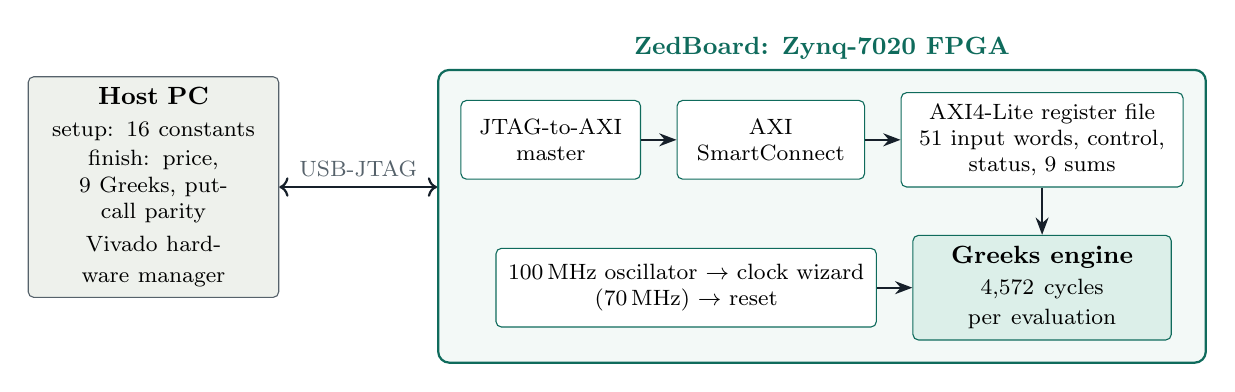
\begin{tikzpicture}[node distance=0.45cm]
  \node[hostb, text width=2.9cm, minimum height=2.8cm] (pc) {\textbf{Host PC}\\[2pt]
    \footnotesize setup: 16 constants\\[1pt] finish: price, 9 Greeks, put-call parity\\[1pt] Vivado hardware manager};
  \node[blk, right=2.3cm of pc, yshift=0.6cm, text width=2.0cm, font=\footnotesize] (jtag) {JTAG-to-AXI\\master};
  \node[blk, right=of jtag, text width=2.1cm, font=\footnotesize] (sc) {AXI\\SmartConnect};
  \node[blk, right=of sc, text width=3.3cm, font=\footnotesize] (reg) {AXI4-Lite register file\\51 input words, control,\\status, 9 sums};
  \node[key, below=0.6cm of reg, text width=3.0cm, minimum height=1.25cm] (eng) {Greeks engine\\\normalfont\footnotesize 4,572 cycles per evaluation};
  \node[blk, left=of eng, text width=4.55cm, font=\footnotesize] (clk) {100\,MHz oscillator $\rightarrow$ clock wizard\\(70\,MHz) $\rightarrow$ reset};
  \draw[arr] (jtag) -- (sc);
  \draw[arr] (sc) -- (reg);
  \draw[arr] (reg) -- (eng);
  \draw[arr] (clk) -- (eng);
  \begin{scope}[on background layer]
    \node[draw=accent, thick, rounded corners=4pt, fill=accentsoft!35, fit=(jtag)(sc)(reg)(eng)(clk), inner sep=8pt,
          label={[font=\small\bfseries, text=accent]above:ZedBoard: Zynq-7020 FPGA}] (fpga) {};
  \end{scope}
  \draw[arr, <->] (pc.east) -- node[lbl, above] {USB-JTAG} (pc.east -| fpga.west);
\end{tikzpicture}
\caption{The system built on the ZedBoard (Vivado block design). The engine is driven
over the JTAG cable, so the test exercises the datapath alone, with no processor
software in the loop.}
\label{fig:board}
\end{figure}

\subsection{Inside the engine}
\textbf{Arithmetic.} The engine has no dividers. Reciprocals and square roots use
Newton-Raphson iterations seeded from small tables, the exponential uses Tang's
method, the logarithm a table and a short series, and sine and cosine a CORDIC unit.
As a result every COS term costs exactly 250 multiplications, 3 CORDIC rotations and
2 CORDIC vectorings, and all of it runs on \textbf{8 shared 56-bit multipliers} and
\textbf{5 CORDIC units}.

\textbf{Per term} (Figure~\ref{fig:term}), the forward pass evaluates the payoff
coefficient and the characteristic function; the reverse sweep then propagates
adjoints back to the model inputs, reusing the forward pass's reciprocals; a
power-of-two normalisation keeps the small adjoints of high-frequency terms at full
precision; and nine accumulators sum the price and Greek contributions.

\begin{figure}[H]
\centering
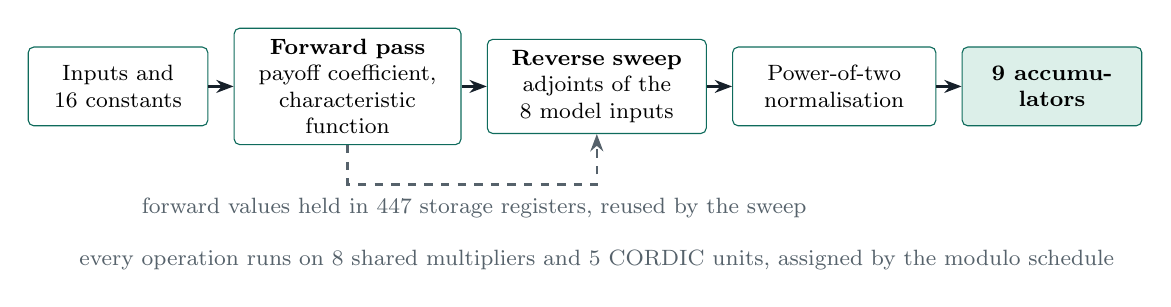
\begin{tikzpicture}[node distance=0.32cm]
  \node[blk, text width=2.0cm, font=\footnotesize] (in) {Inputs and\\16 constants};
  \node[blk, right=of in, text width=2.6cm, font=\footnotesize] (fwd) {\textbf{Forward pass}\\payoff coefficient,\\characteristic function};
  \node[blk, right=of fwd, text width=2.5cm, font=\footnotesize] (rev) {\textbf{Reverse sweep}\\adjoints of the\\8 model inputs};
  \node[blk, right=of rev, text width=2.3cm, font=\footnotesize] (nrm) {Power-of-two\\normalisation};
  \node[key, right=of nrm, text width=2.0cm, font=\footnotesize\bfseries] (acc) {9 accumu-\\lators};
  \draw[arr] (in) -- (fwd);
  \draw[arr] (fwd) -- (rev);
  \draw[arr] (rev) -- (nrm);
  \draw[arr] (nrm) -- (acc);
  \draw[darr] (fwd.south) -- ++(0,-0.5) -| (rev.south);
  \node[lbl, below=0.55cm of fwd.south east, xshift=0.16cm] {forward values held in 447 storage registers, reused by the sweep};
  \node[lbl, below=1.35cm of rev.south] {every operation runs on 8 shared multipliers and 5 CORDIC units, assigned by the modulo schedule};
\end{tikzpicture}
\caption{One COS term inside the engine. The adjoint sweep is part of the same
datapath as the forward pass; there is no tape memory.}
\label{fig:term}
\end{figure}

\textbf{Schedule.} The 128 terms are independent, so a new term starts every
\emph{initiation interval} of 32 cycles while earlier terms are still in flight
(Figure~\ref{fig:sched}). At 8 multipliers, 3 rotation and 2 vectoring units, all
three resource classes give the same interval:
$\lceil 250/8 \rceil = 32$ and $3\times32/3 = 2\times32/2 = 32$. One evaluation takes
$127\times32 + 506 + 2 = 4{,}572$ cycles on the FPGA. Because the CORDIC units set the
pace, the forward pass leaves multiplier slots idle in every 32-cycle window; the
reverse sweep's multiplications fill them, which is why the nine Greeks cost almost
nothing.

\begin{figure}[H]
\centering
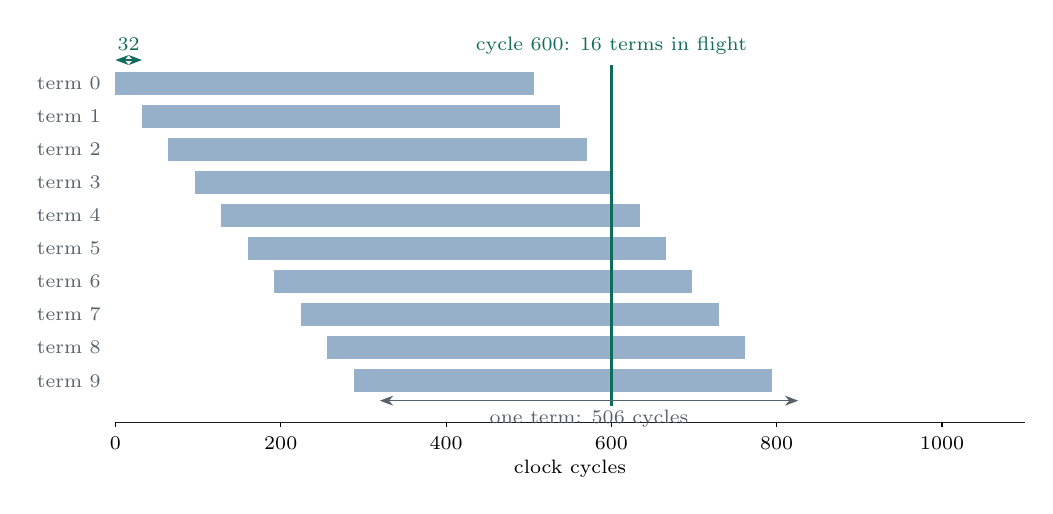
\begin{tikzpicture}[x=0.0105cm, y=0.42cm]
  \foreach \k in {0,...,9} {
    \pgfmathsetmacro{\s}{\k*32}
    \fill[plan!80] (\s, -\k) rectangle ++(506, 0.7);
    \node[font=\scriptsize, text=muted, anchor=east] at (-6, -\k+0.35) {term $\k$};
  }
  \draw[accent, very thick] (600,-9.4) -- (600,0.9) node[above, font=\scriptsize, text=accent] {cycle 600: 16 terms in flight};
  \draw[ink] (0,-9.9) -- (1100,-9.9);
  \foreach \c in {0,200,400,600,800,1000} { \draw (\c,-9.9) -- ++(0,-0.15) node[below, font=\scriptsize] {\c}; }
  \node[font=\scriptsize] at (550,-11.3) {clock cycles};
  \draw[{Stealth}-{Stealth}, accent] (0,1.05) -- node[above, font=\scriptsize, text=accent] {32} (32,1.05);
  \draw[{Stealth}-{Stealth}, muted] (320,-9.25) -- node[below, font=\scriptsize, text=muted] {one term: 506 cycles} (826,-9.25);
\end{tikzpicture}
\caption{The modulo schedule (first ten of 128 terms). A term lasts 506 cycles and a
new one starts every 32, so about 16 terms share the arithmetic units at any time.}
\label{fig:sched}
\end{figure}

\textbf{Precision.} The datapath uses 56-bit fixed-point words with 28 fractional
bits, rounding to nearest at every step. An FPGA has no fixed word length: adders and
multipliers are built at whatever width the design needs, and a 56$\times$56-bit
multiplier is assembled from nine of the chip's 25$\times$18-bit DSP blocks (72 DSP
blocks for the 8 multipliers). Section~\ref{sec:wl} shows why 56 bits. Data-dependent shift amounts were measured
over the valid input range and the shifters built only that wide, which cut logic by
35\%; any input that would exceed a measured range raises a \texttt{range\_err} flag
instead of returning a wrong value.

% =====================================================================
\section{Results}

Table~\ref{tab:glance} summarises the results; each is detailed below with why it
is useful and what is new.

\begin{table}[H]
\centering
\small
\begin{tabularx}{\textwidth}{@{}l Y Y@{}}
\toprule
\textbf{Measure} & \textbf{Result} & \textbf{Compared with}\\
\midrule
Cycles, price + 9 Greeks & 4,733 & 92$\times$ fewer than the first-generation engine; 18.4$\times$ fewer than bump-and-reprice\\
Cost of the 9 Greeks & 1.04 pricings & hand-derived software 1.9; AD tools 5.3--6.7; bump-and-reprice 19\\
Latency on the ZedBoard (loop only) & 65.3\,$\mu$s (57.8\,$\mu$s at 79\,MHz) & 1.4--3.9$\times$ faster than AD tools and bumping on one CPU core; 2.2$\times$ slower than hand-derived Greeks (29\,$\mu$s)\\
Energy per evaluation & 22.2\,$\mu$J & about 6--30$\times$ less than the CPU (CPU power estimated)\\
Accuracy (21 cases) & price $6.1\times10^{-7}$, Greeks $\le 1.2\times10^{-5}$ & relative to double precision; over 10,500 inputs worst absolute $1.2\times10^{-3}$ ($\partial V/\partial\xi$)\\
Error bound & never exceeded ($\le 0.378$) & every output, 10,500 inputs\\
On silicon & 450 / 450 bit-exact & 50 random cases\\
Area & 73\% LUT, 72 of 220 DSP & fits a Zynq-7020; the first generation did not\\
\bottomrule
\end{tabularx}
\caption{Results at a glance (Zynq-7020 configuration).}
\label{tab:glance}
\end{table}

\subsection{Speed: clock cycles for the price and nine Greeks}
\begin{table}[H]
\centering
\small
\resizebox{\textwidth}{!}{\begin{tabular}{@{}lrrrrr@{}}
\toprule
\textbf{Design} & \textbf{Price + 9 Greeks} & \textbf{Price only} & \textbf{Bump-and-reprice} & \textbf{Bump $\div$ adjoint} & \textbf{Greeks cost}\\
\midrule
First generation (hand-written, 64-bit) & 433,779 & 200,562 & 3,811,647 & 8.8$\times$ & 2.16$\times$\\
\hi Generated, Zynq-7020 (56-bit, 8 multipliers) & \textbf{4,733} & 4,568 & 86,860 & \textbf{18.4$\times$} & \textbf{1.04$\times$}\\
Generated, board design (loop on FPGA) & 4,572 & -- & -- & -- & --\\
Generated, 64-bit (32 multipliers) & 1,593 & 1,026 & 19,562 & 12.3$\times$ & 1.55$\times$\\
\bottomrule
\end{tabular}}
\caption{Clock cycles per evaluation, from cycle-exact RTL simulation (128 COS terms).
``Greeks cost'' is the price-with-Greeks cycles divided by the price-only cycles on
the same hardware.}
\label{tab:cycles}
\end{table}

\begin{figure}[H]
\centering
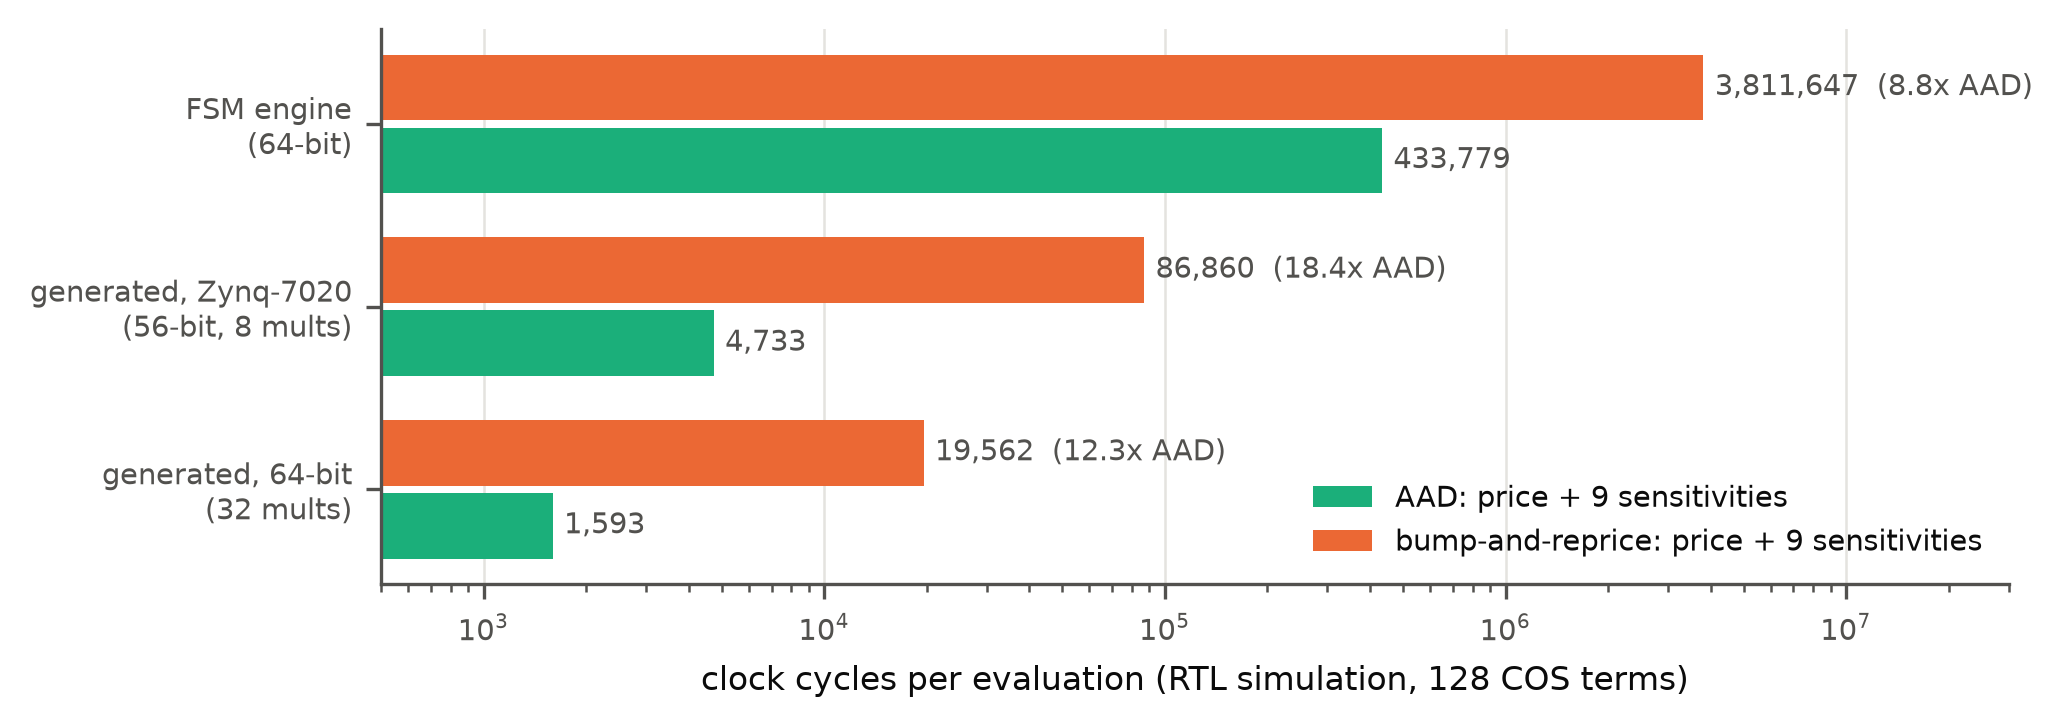
\includegraphics[width=\textwidth]{figures/fig8_architecture_cycles.png}
\caption{Cycles per evaluation, adjoint against bump-and-reprice on the same hardware
(log scale).}
\end{figure}

\useful{A full risk report for one option, price and nine Greeks, costs only 3.6\%
more than its price alone: 165 extra cycles. Risk can be recomputed as often as
prices, instead of 18.4 times less often under bump-and-reprice.}
\novel{No hardware had computed Greeks by adjoint differentiation before, so no
hardware had shown this cost. Software adjoint differentiation costs 5.3--6.7
pricings because of its tape; here the reverse sweep fills idle multiplier slots
left by the CORDIC-bound forward pass. A forward-mode sweep could fill them too, but
needs more multiplies (Section~\ref{sec:modes}). On the 64-bit design, where
multipliers are the bottleneck, the cost is 1.55 pricings, which is still well below
software.}

\subsection{Design space: cycles against hardware size}
\begin{table}[H]
\centering
\small
\resizebox{\textwidth}{!}{\begin{tabular}{@{}lrrrrrr@{}}
\toprule
\textbf{Configuration} & \textbf{Multipliers} & \textbf{Interval} & \textbf{Price + Greeks} & \textbf{Price only} & \textbf{Bump} & \textbf{Bump $\div$ adjoint}\\
\midrule
Zynq-7020 (56-bit) & 2 & 125 & 16,754 & 8,700 & 165,368 & 9.9\\
Zynq-7020 (56-bit) & 4 & 63 & 8,694 & 4,613 & 87,715 & 10.1\\
\hi Zynq-7020 (56-bit) & 8 & 32 & 4,733 & 4,568 & 86,860 & 18.4\\
Zynq-7020 (56-bit) & 16 & 32 & 4,621 & 4,563 & 86,765 & 18.8\\
64-bit & 1 & 250 & 32,530 & 16,773 & 318,755 & 9.8\\
64-bit & 4 & 63 & 8,700 & 4,636 & 88,152 & 10.1\\
64-bit & 8 & 32 & 4,709 & 2,573 & 48,955 & 10.4\\
64-bit & 16 & 16 & 2,614 & 1,540 & 29,328 & 11.2\\
\hi 64-bit & 32 & 8 & 1,593 & 1,026 & 19,562 & 12.3\\
64-bit & 64 & 4 & 1,073 & 888 & 16,940 & 15.8\\
64-bit & 128 & 3 & 942 & 888 & 16,940 & 18.0\\
\bottomrule
\end{tabular}}
\caption{Cycles per evaluation as the number of shared multipliers changes. The
interval is the number of cycles between the starts of consecutive COS terms.}
\end{table}

\begin{figure}[H]
\centering
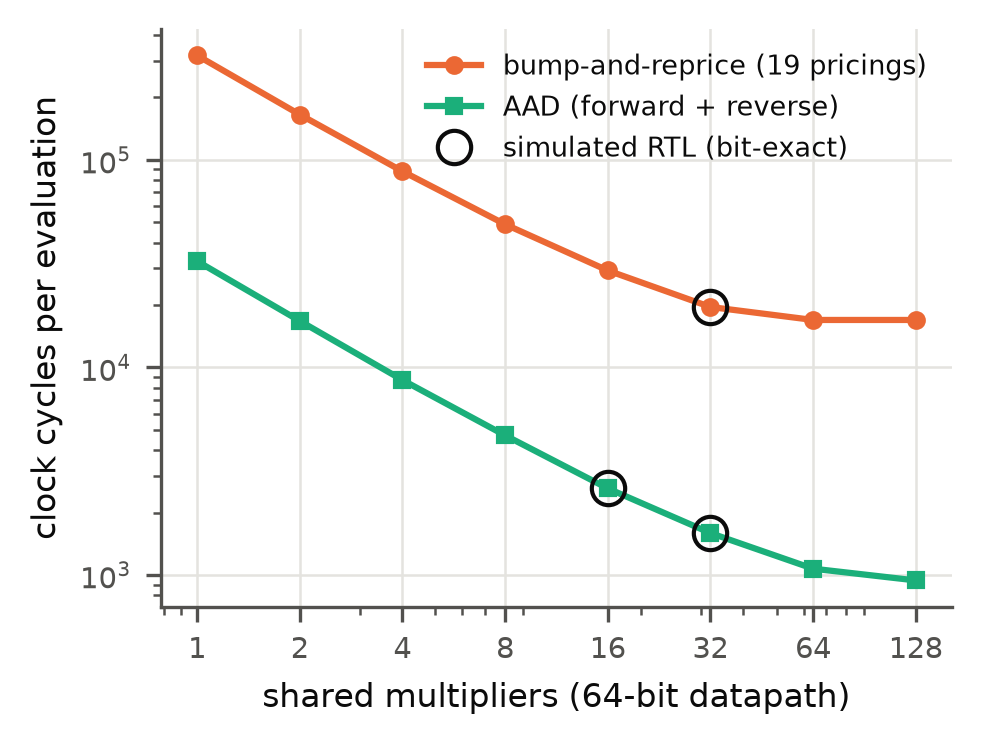
\includegraphics[width=0.62\textwidth]{figures/fig9_cycles_vs_mults.png}
\caption{Cycles against shared multipliers (64-bit). Circled points were simulated as
RTL and matched the schedule exactly.}
\end{figure}

\useful{The same generator produces a small engine for a low-cost FPGA or a fast one
for a large FPGA from one parameter. Cycles halve as multipliers double until another
resource sets the pace; at 8 multipliers on the Zynq-7020 design the CORDIC units do,
so a 16th multiplier gains only 2\%. The table shows where extra hardware stops paying.}

\subsection{Adjoint against forward mode on the same hardware}
\label{sec:modes}
The reverse sweep is not the only way to get all nine Greeks in one evaluation. Three
forward-mode (tangent) datapaths were built by the same generator, from the same
primitives, with the same frozen truncation range, hoisting and finish, and scheduled by
the same scheduler: \emph{dense}, which carries all eight input directions through every
operation as a vector forward-mode AD tool does; \emph{sparse}, which skips derivatives
that are structurally zero; and \emph{factored}, which forms the derivatives of the
characteristic-function exponent with respect to its two complex inner quantities and
the maturity once per term and combines them for each Greek, as a careful hand
derivation of analytic Greeks does (Cui et al.~\cite{cui}). All three return the same
price and Greeks as the adjoint datapath to within $6\times10^{-14}$ in double
precision.

\begin{table}[H]
\centering
\small
\resizebox{\textwidth}{!}{\begin{tabular}{@{}lrrrrr@{}}
\toprule
& & \multicolumn{2}{c}{\textbf{Zynq-7020 (56-bit)}} & \multicolumn{2}{c}{\textbf{64-bit}}\\
\textbf{Datapath} & \textbf{Multiplies per term} & \textbf{8 mult.} & \textbf{16 mult.} & \textbf{16 mult.} & \textbf{32 mult.}\\
\midrule
Price only & 126 & 4,566 & 4,561 & 1,538 & 1,024\\
\hi Adjoint (this work) & \textbf{250} & \textbf{4,731} & 4,619 & \textbf{2,612} & \textbf{1,591}\\
Forward, factored (analytic) & 313 & 5,622 & 4,571 & 3,069 & 1,795\\
Forward, sparse & 396 & 6,968 & 4,571 & 3,690 & 2,171\\
Forward, dense (AD tool) & 802 & 13,597 & 7,150 & 7,155 & 3,822\\
\bottomrule
\end{tabular}}
\caption{Multiplies per COS term and cycles per evaluation for the price and nine
Greeks, by datapath and number of shared multipliers
(\texttt{validation/run\_mode\_baselines.py}). The forward datapaths have no
fixed-point rescaling of their tangents, which a working engine would need, so their
counts are lower bounds.}
\label{tab:modes}
\end{table}

\useful{For the same Greeks, the adjoint needs the fewest multiplies: 124 per term
beyond the price, against 187 for the best hand-factored forward method and 676 for
forward mode as an AD tool builds it. With the board's 8 multipliers that is 4,731
cycles against 5,622 and 13,597. The 1.04 pricings of Table~\ref{tab:cycles} are not
unique to the adjoint: with 16 multipliers the CORDIC units set the pace for every
variant except the dense one, and all reach about 4,570 cycles. What the adjoint saves
is hardware: it reaches that pace with 8 multipliers (72 DSP blocks), where the
factored forward method needs 10 (90) and the dense one 26 (234, more than the chip
has).}

\subsection{Accuracy and the first-order error bound}
\begin{table}[H]
\centering
\small
\begin{tabular}{@{}lccc@{}}
\toprule
\textbf{Output} & \textbf{Zynq-7020 (56-bit)} & \textbf{64-bit} & \textbf{Worst error $\div$ bound}\\
\midrule
Price & $6.1\times10^{-7}$ & $2.8\times10^{-8}$ & 0.074\\
Delta $\partial V/\partial S_0$ & $2.0\times10^{-7}$ & $6.9\times10^{-9}$ & 0.049\\
$\partial V/\partial K$ & $2.5\times10^{-7}$ & $6.6\times10^{-9}$ & 0.051\\
$\partial V/\partial T$ & $3.1\times10^{-7}$ & $6.0\times10^{-9}$ & 0.093\\
Rho $\partial V/\partial r$ & $2.4\times10^{-7}$ & $8.9\times10^{-9}$ & 0.049\\
Vega $\partial V/\partial v_0$ & $6.2\times10^{-7}$ & $2.0\times10^{-8}$ & 0.103\\
$\partial V/\partial\kappa$ & $7.8\times10^{-6}$ & $4.1\times10^{-7}$ & 0.098\\
$\partial V/\partial\theta$ & $7.9\times10^{-7}$ & $3.4\times10^{-8}$ & 0.102\\
$\partial V/\partial\xi$ & $2.7\times10^{-6}$ & $2.2\times10^{-7}$ & 0.099\\
$\partial V/\partial\rho$ & $1.2\times10^{-5}$ & $7.4\times10^{-7}$ & 0.087\\
\bottomrule
\end{tabular}
\caption{Worst relative error over 21 parameter sets (moneyness, maturity, vol-of-vol,
correlation; calls and puts) against the double-precision model, and the largest
measured error as a fraction of the first-order bound, across both designs.}
\label{tab:acc}
\end{table}

\begin{figure}[H]
\centering
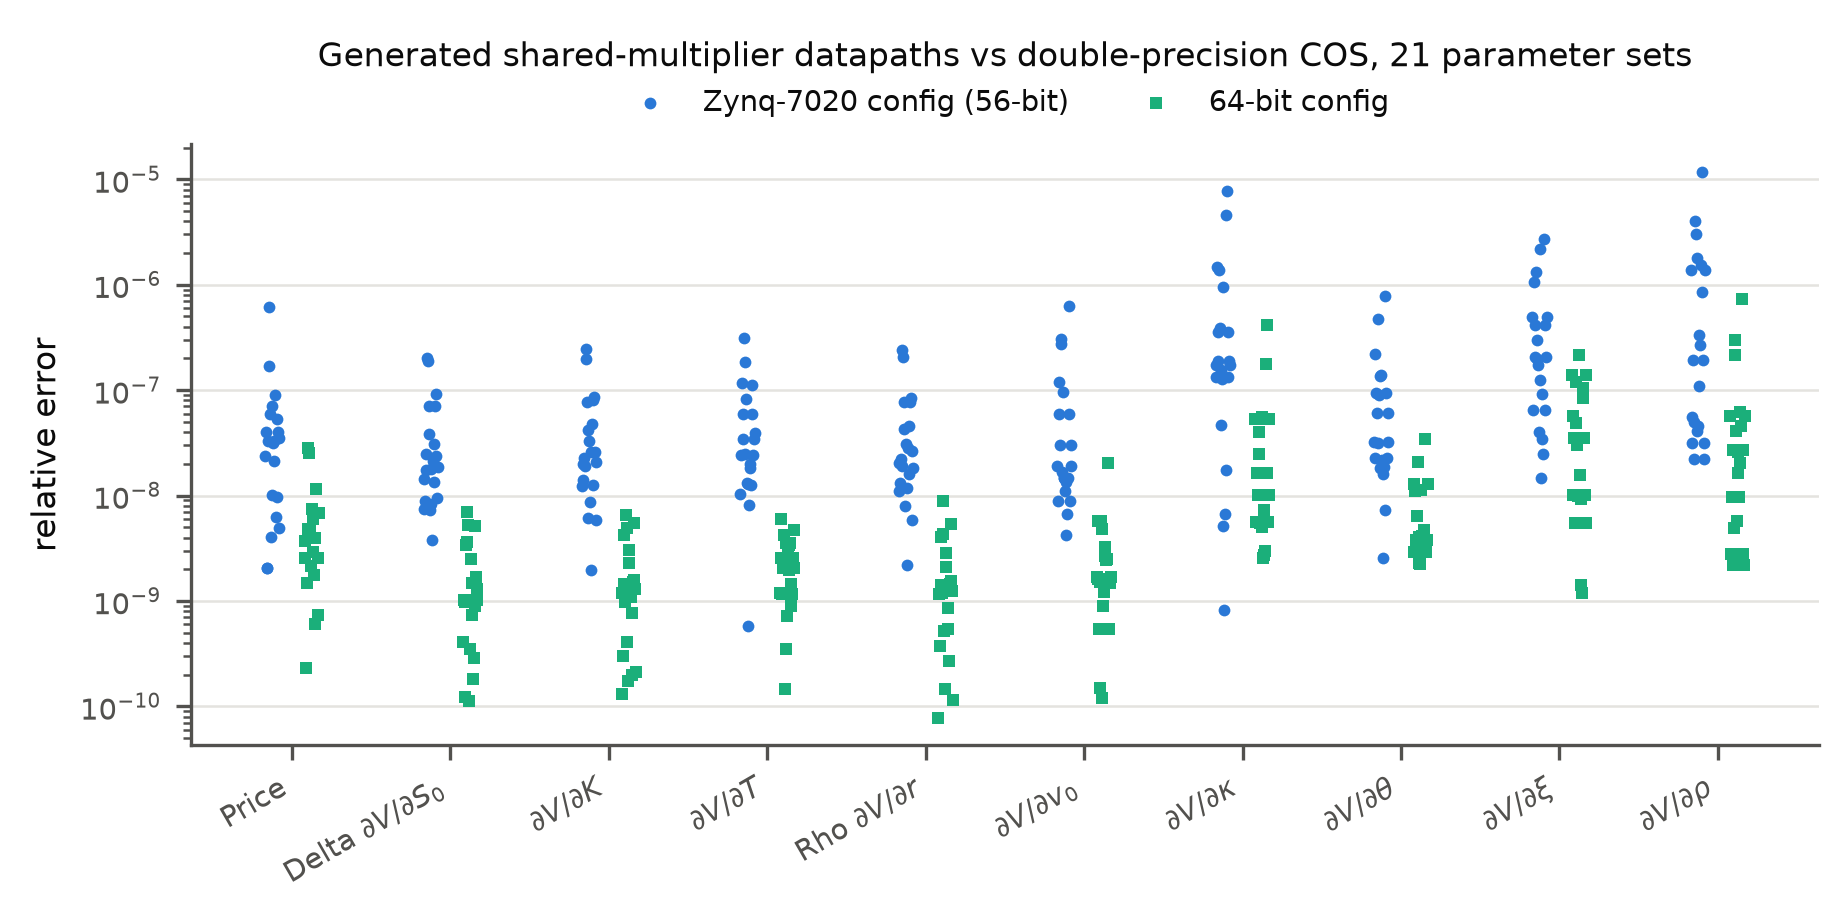
\includegraphics[width=\textwidth]{figures/fig11_gen_accuracy.png}
\caption{Relative error of every output for both designs over the 21 parameter sets.}
\end{figure}

A larger sweep tested the 56-bit design on 10,500 inputs: 6,000 uniform over the verified
domain, 500 in each of seven hard regimes (Feller condition violated, correlation near its
limits, deep strikes, very short and long maturities, high vol-of-vol, very low variance)
and 1,000 with one input outside the domain. Each case runs the bit-accurate model, the
error bound, the reference, and the same range check that raises the hardware's
\texttt{range\_err} flag.

\begin{table}[H]
\centering
\small
\begin{tabular}{@{}lrrr@{}}
\toprule
\textbf{Output (absolute error)} & \textbf{Median} & \textbf{99th percentile} & \textbf{Worst}\\
\midrule
Price & $3.3\times10^{-7}$ & $1.7\times10^{-5}$ & $7.3\times10^{-5}$\\
Delta & $3.5\times10^{-9}$ & $1.6\times10^{-7}$ & $2.2\times10^{-6}$\\
Vega $\partial V/\partial v_0$ & $2.8\times10^{-7}$ & $2.1\times10^{-5}$ & $2.9\times10^{-4}$\\
$\partial V/\partial\theta$ & $2.0\times10^{-6}$ & $1.1\times10^{-4}$ & $3.7\times10^{-4}$\\
$\partial V/\partial\xi$ & $5.9\times10^{-7}$ & $2.5\times10^{-4}$ & $1.3\times10^{-3}$\\
\bottomrule
\end{tabular}
\caption{56-bit design, all 9,500 in-domain inputs.}
\end{table}

No result exceeded its error bound in any of the 10,482 unflagged cases, inside or
outside the domain (worst 0.378 of the bound), with no overflow; the 18 flagged inputs
were all outside the domain. The 21-case grid understates the tail: at small vol-of-vol
($\xi\approx0.1$) with large $\kappa\theta$, $\partial V/\partial\xi$ is off by up to
$1.3\times10^{-3}$, all of it fixed-point rounding and inside its bound. The sweep also exposed false alarms: \texttt{range\_err} fired on 25
in-domain inputs at very low variance and very short maturity, where two normalization
shifts went one step past their fitted range. Fitting the ranges on extra samples at
the ten edges of the domain widened 50 of 113 shifters by 1--4 steps and removed every
in-domain flag; all designs were regenerated and pass their bit-exact testbenches.
Because that sweep had prompted the refit, the refitted ranges were then tested on a
fresh, held-out sweep of the same size (seed 20261006, \texttt{run\_domain\_sweep.py
--heldout}): none of its 9,500 in-domain inputs raised \texttt{range\_err}, none
exceeded its bound (worst 0.356 of it), and of the 1,000 out-of-domain inputs 9 were
flagged and every other one stayed within its bound.

\useful{The error bound is reliable over ten thousand inputs, including the hard regimes:
every result the hardware does not flag is within its computed bound, so a user knows
each Greek's accuracy before using it, and no valid input is now rejected.}

\useful{Against the same algorithm in double precision, over the 9,500 held-out
in-domain inputs, the price, delta, strike sensitivity, theta, rho and vega are good to
at least 5.3 significant figures in 99\% of inputs (median 7.6--8.1; worst 3.3--4.4).
The model-parameter sensitivities are weaker: $\partial V/\partial\theta$ and
$\partial V/\partial\rho$ give 4.9 figures at the 99th percentile, and
$\partial V/\partial\kappa$ and $\partial V/\partial\xi$ only 3.5 and 3.0, falling to
2.2 and 1.4 where they are small (\texttt{validation/sigfig\_report.py}; inputs where a
Greek is within 1\% of zero are excluded). Each result comes with a bound computed in
0.1\,s per parameter set that the hardware error never exceeded. A risk system can rely on the bound instead of on the cases that
happened to be tested.}
\novel{FPGA finance work validates fixed point by measuring error over test cases.
Here a rounding-error bound is computed for every Greek produced by the adjoint
datapath, because the error model includes the hardware's own reverse sweep.
Measured error reaches at most 0.103 of the bound.}

\paragraph{What the bound covers.} The bound is first order: it propagates every
rounding error through the derivatives of the computation and drops products of
rounding errors, which are smaller by a factor of about $2^{-28}$ at this word length.
It covers fixed-point rounding only, measured against the same algorithm computed
exactly; the COS method's own truncation error is a separate term
(Section~\ref{sec:methoderr}). Two checks support dropping the second-order terms.
First, the same graph was evaluated in 50-digit arithmetic on 100 held-out inputs
(\texttt{validation/run\_mp\_check.py}): the hardware's error against the 50-digit value
is at most 0.24 of the bound, the same to three decimals as against double precision,
and double precision itself is within $5\times10^{-5}$ of the bound from the exact value.
Second, the bound still held at 44 bits (Section~\ref{sec:wordlength}), where
second-order terms are relatively 4,096 times larger than at 56 bits.

\subsection{COS truncation error: a separate term}
\label{sec:methoderr}
The engine computes the COS approximation of the Heston price: 128 terms over a
truncation range of $\pm10$ standard deviations. Its distance from the exact Heston
value is the method's own error, which no word length removes. On the 50 board cases it
was measured against an independent Fourier-integral reference
(\texttt{validation/run\_method\_error.py}).

\begin{table}[H]
\centering
\small
\begin{tabular}{@{}lrrrr@{}}
\toprule
\textbf{Output} & \textbf{Method error, median} & \textbf{Method error, worst} & \textbf{Rounding, worst} & \textbf{Rounding bound, worst}\\
\midrule
Price & $2.1\times10^{-11}$ & $4.4\times10^{-5}$ & $1.5\times10^{-5}$ & $2.8\times10^{-4}$\\
Delta & $6.9\times10^{-10}$ & $8.3\times10^{-5}$ & $1.1\times10^{-7}$ & $1.6\times10^{-6}$\\
Vega & $1.3\times10^{-9}$ & $7.8\times10^{-3}$ & $1.4\times10^{-5}$ & $2.0\times10^{-4}$\\
$\partial V/\partial\theta$ & $5.6\times10^{-9}$ & $2.5\times10^{-3}$ & $7.0\times10^{-5}$ & $1.8\times10^{-3}$\\
$\partial V/\partial\xi$ & $1.3\times10^{-9}$ & $1.8\times10^{-3}$ & $2.1\times10^{-4}$ & $4.5\times10^{-3}$\\
\bottomrule
\end{tabular}
\caption{Absolute errors over the 50 board cases. Method error: COS (128 terms, double
precision) against the Fourier integral. Rounding: the board's results against COS in
double precision. The other outputs behave alike.}
\label{tab:methoderr}
\end{table}

In a typical case the method error is far below the rounding error, but in a few it is
much larger. The five worst cases have two causes. In three, 128 terms are too few (high
volatility of volatility with short maturity: $\xi = 1$, $T = 0.34$ gives the worst vega
error); with 256 terms COS matches the integral. In two, the truncation range is
too narrow (a deep out-of-the-money put); a range 1.5 times wider matches the integral.
The total error of a result against the Heston model is at most the rounding bound plus
the method error, and only the first is bounded.

\useful{Separating the two terms shows where accuracy is lost. Rounding is bounded and
small; the method error comes from the choice of 128 terms and the range rule, which
any implementation of this COS configuration shares, in hardware or software. Where it
matters, more terms (256 roughly doubles the cycles) or a wider range would reduce it.}

\subsection{Accuracy against bump-and-reprice}
\begin{figure}[H]
\centering
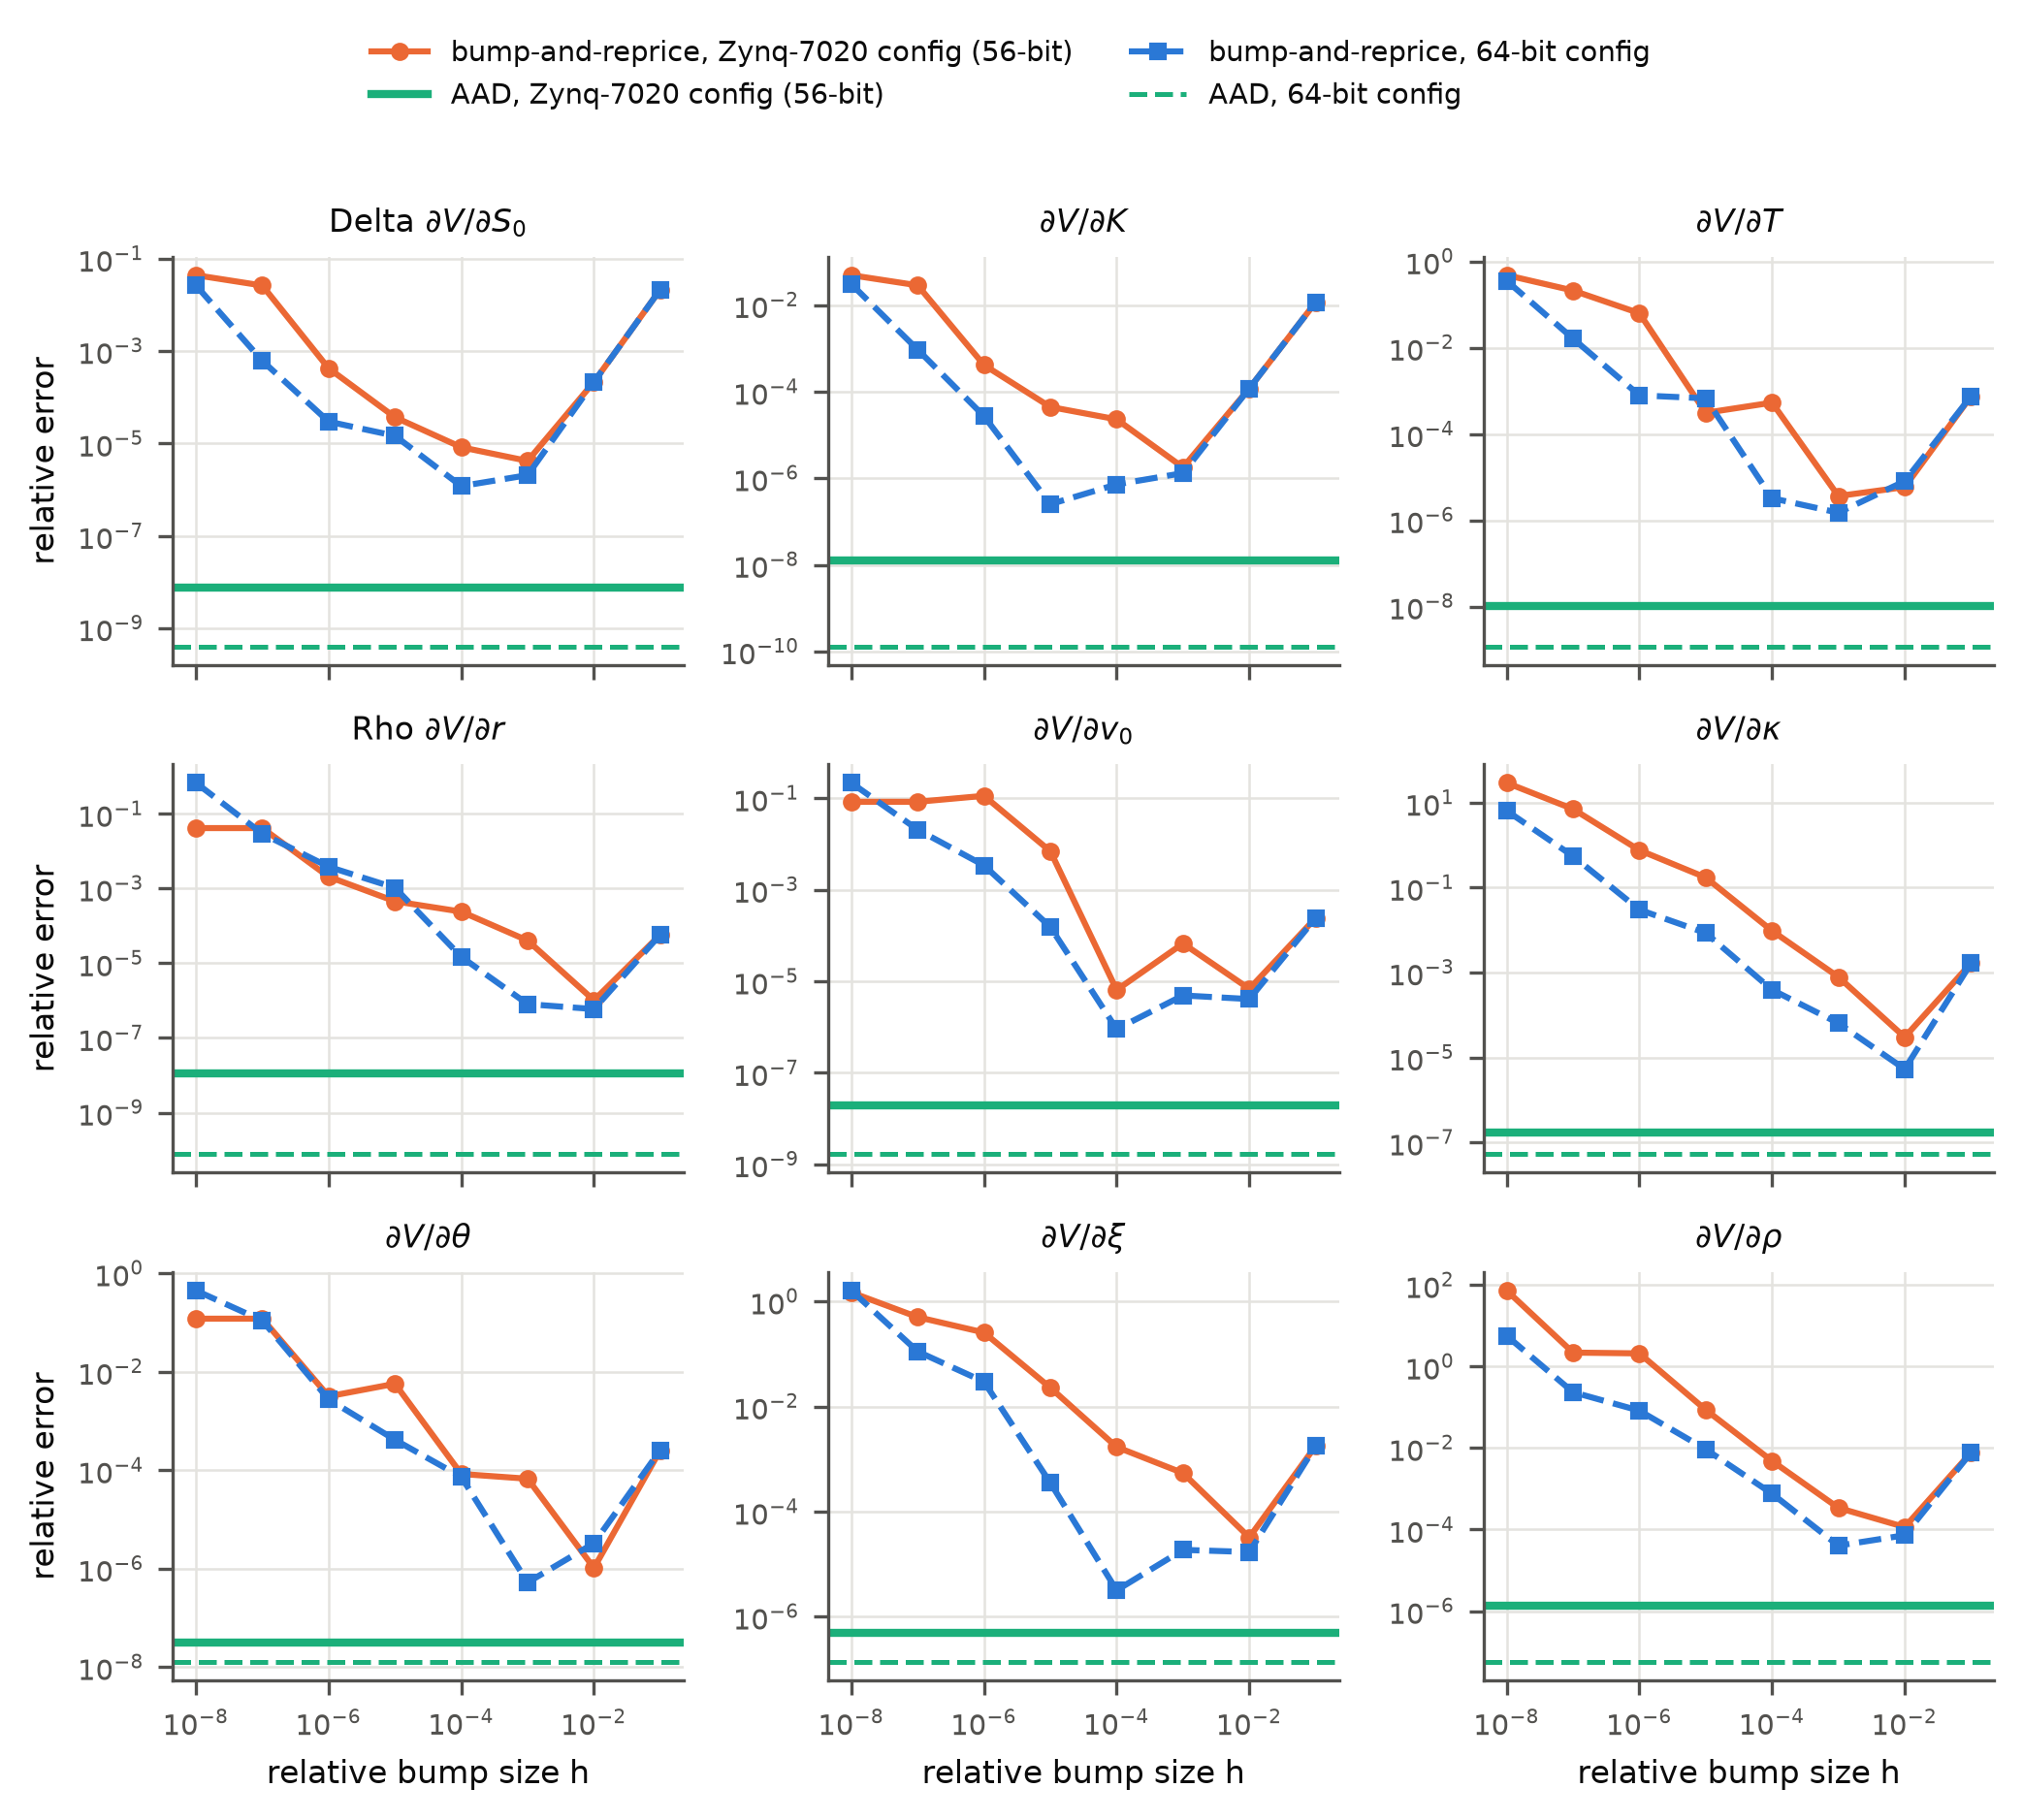
\includegraphics[width=0.92\textwidth]{figures/fig10_gen_bump_vs_aad.png}
\caption{Every Greek: bump-and-reprice error against bump size (curves) and the
adjoint engine (flat lines), on the same pricer and word length.}
\end{figure}

\useful{Bump-and-reprice error is U-shaped in the bump size and has no setting that is
safe for every Greek. On the Zynq-7020 design the adjoint Greeks are 32--560 times
more accurate than bump-and-reprice even with the best bump size chosen afterwards for
each Greek (median 145 times), with nothing to tune.}

\subsection{Accuracy against word length}
\label{sec:wordlength}
\label{sec:wl}
\begin{table}[H]
\centering
\small
\resizebox{\textwidth}{!}{\begin{tabular}{@{}lcccc@{}}
\toprule
\textbf{Word length (fraction bits)} & \textbf{Worst price error} & \textbf{Worst Greek error} & \textbf{Worst error $\div$ bound} & \textbf{Overflows}\\
\midrule
44-bit (16) & $1.5\times10^{-3}$ & $2.8\times10^{-1}$ & 0.167 & 0\\
48-bit (20) & $1.8\times10^{-4}$ & $9.1\times10^{-3}$ & 0.121 & 0\\
52-bit (24) & $5.0\times10^{-6}$ & $5.8\times10^{-4}$ & 0.113 & 0\\
\hi 56-bit (28), this design & $6.1\times10^{-7}$ & $1.2\times10^{-5}$ & 0.103 & 0\\
64-bit (32) & $2.8\times10^{-8}$ & $7.4\times10^{-7}$ & 0.099 & 0\\
64-bit (36) & $1.2\times10^{-9}$ & $7.9\times10^{-8}$ & 0.150 & 0\\
\bottomrule
\end{tabular}}
\caption{Worst relative error over the 21 parameter sets as the word length changes
(\texttt{validation/results/wordlength\_sweep.csv}).}
\end{table}

\useful{Every four bits removed costs roughly 10--50 times in Greek accuracy. At 48 bits
a Greek can be 1\% wrong and at 44 bits 28\% wrong, while 64 bits buys accuracy no risk
desk needs at a higher hardware cost; at 56 bits the price and the market Greeks are
good to at least five significant figures in 99\% of inputs, and the model-parameter
sensitivities to at least three. The first-order bound held at every width, so it predicts this
trade-off without building each design.}

\subsection{Calls through put-call parity}
\label{sec:parity}
Priced directly, a call's COS coefficients contain $e^{b}$ for the upper truncation
bound $b$, which grows large over a wide range and then cancels, losing precision in
fixed point. The engine now always prices the put and adds
$S_0 - K e^{-rT}$ and its derivatives for a call.

\begin{table}[H]
\centering
\small
\begin{tabular}{@{}lrrr@{}}
\toprule
\textbf{Worst absolute error, 22 calls} & \textbf{Call priced directly} & \textbf{Put + parity} & \textbf{Improvement}\\
\midrule
\hi Price & $2.3\times10^{-3}$ & $3.1\times10^{-5}$ & 75$\times$\\
Price (median) & $4.8\times10^{-5}$ & $5.4\times10^{-7}$ & $\approx$90$\times$\\
$\partial V/\partial\kappa$ & $2.4\times10^{-3}$ & $3.9\times10^{-4}$ & 6$\times$\\
$\partial V/\partial\theta$ & $1.7\times10^{-2}$ & $2.5\times10^{-3}$ & 7$\times$\\
$\partial V/\partial\xi$ & $1.3\times10^{-2}$ & $1.8\times10^{-3}$ & 7$\times$\\
$\partial V/\partial\rho$ & $8.3\times10^{-3}$ & $4.7\times10^{-4}$ & 18$\times$\\
Delta, $\partial V/\partial K$, $\partial V/\partial T$, rho, vega & & & 2--2.5$\times$\\
\bottomrule
\end{tabular}
\caption{Effect of put-call parity on the 22 calls of the 50-case board set, against
the independent Fourier-integral price. It costs 2 cycles (4,731 $\rightarrow$ 4,733)
and removes one multiplication per term.}
\end{table}

\useful{The worst call price error falls 75-fold, and every Greek improves. After the
change, the hardware's error matches the error of the COS method itself, so fixed-point
rounding is no longer the limiting factor.}

\subsection{Implementation on the Zynq-7020}
\begin{table}[H]
\centering
\small
\resizebox{\textwidth}{!}{\begin{tabular}{@{}lrrrrrr@{}}
\toprule
\textbf{Build} & \textbf{LUT} & \textbf{FF} & \textbf{DSP} & \textbf{Clock} & \textbf{Slack} & \textbf{Power}\\
\midrule
Engine alone (xc7z020clg400-1) & 36,499 (68.6\%) & 28,559 (26.8\%) & 72 (32.7\%) & 100\,MHz & $-2.639$\,ns & 0.258\,W\\
\hi ZedBoard system (xc7z020clg484-1) & 38,752 (72.8\%) & 32,134 (30.2\%) & 72 (32.7\%) & 70\,MHz & $+0.458$\,ns & 0.340\,W\\
\bottomrule
\end{tabular}}
\caption{Vivado 2025.2 results after routing. The engine alone reaches about 79\,MHz;
inside the board system the design meets timing at 70\,MHz. Power is Vivado's power
report (vectorless analysis); 0.121\,W of the board figure is the clock generator.}
\end{table}

\begin{figure}[H]
\centering
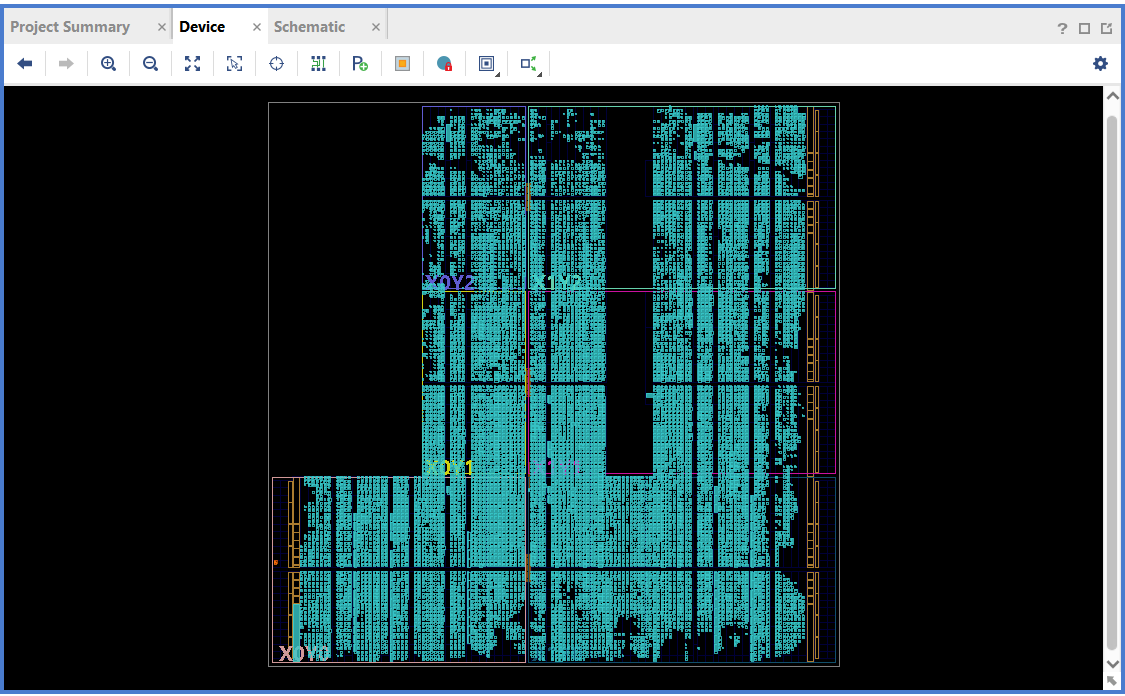
\includegraphics[width=0.58\textwidth]{figures/vivado_device.png}\\[4pt]
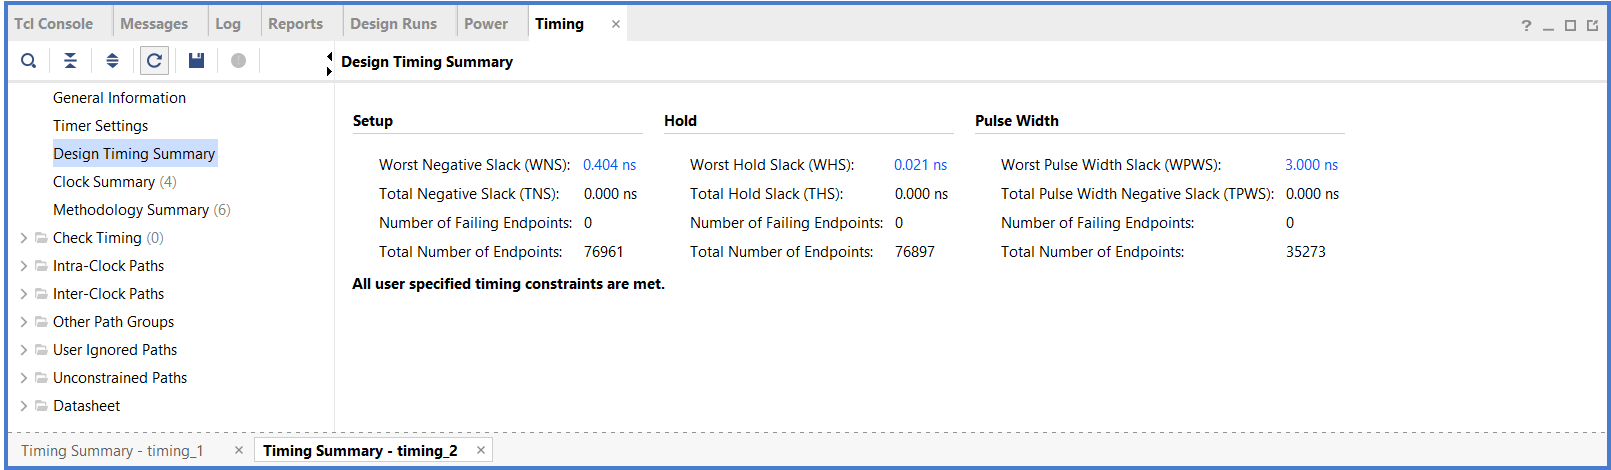
\includegraphics[width=\textwidth]{figures/vivado_timing.png}
\caption{The placed design on the Zynq-7020 (top) and the timing summary of the
ZedBoard build of 29 September: all constraints met at 70\,MHz, 0 failing endpoints of
76,961 (bottom). The rebuild of 6 October with put-call parity and the refitted ranges
also meets 70\,MHz: WNS $+0.458$\,ns, 0 failing endpoints of 76,672, and 394 more LUTs.}
\end{figure}

\useful{The engine fits a low-cost Zynq-7020 with room to spare: 73\% of the logic and
a third of the DSP blocks, leaving space for the processor interface. The first
generation could not fit at all.}

\subsection{On silicon}
\begin{table}[H]
\centering
\small
\begin{tabular}{@{}lrrrr@{}}
\toprule
\textbf{Run} & \textbf{Cases} & \textbf{Bit-exact results} & \textbf{Range errors} & \textbf{Worst error $\div$ bound}\\
\midrule
First vector & 1 & 9 / 9 & 0 & 0.049\\
\hi Sweep, back to back & 50 & 450 / 450 & 0 & 0.199\\
\bottomrule
\end{tabular}
\caption{ZedBoard results, 6 October 2026, with the current design (put-call parity
and refitted shift ranges). The sweep used 2 reference cases and 48 random cases over
the valid input range (22 calls, 28 puts), with no reset between cases. Worst price
error over the 50 cases against the double-precision reference: $1.5\times10^{-5}$,
down from $2.3\times10^{-3}$ with the earlier bitstream of 29 September (which was also
450 / 450 bit-exact, worst 0.268 of the bound).}
\end{table}

\useful{The hardware computes exactly what the model computes, so every accuracy result
and the error bound carry over to the chip. Running the cases back to back also shows
that nothing carries over from one evaluation to the next.}
\novel{These are the first adjoint-differentiated option Greeks computed on an FPGA.}

\subsection{Against a CPU}
The same algorithm was written in C++ (double precision, g++ 13, -O3 -march=native) and
run on an Intel Core i5-1155G7 laptop CPU, with adjoint differentiation by the CoDiPack
tool~\cite{codipack}. Every method matches the reference model (adjoint to
$1.3\times10^{-10}$ relative).

\begin{table}[H]
\centering
\small
\begin{tabular}{@{}lrrr@{}}
\toprule
\textbf{Price + 9 Greeks} & \textbf{$\mu$s per evaluation} & \textbf{Cost vs one price} & \textbf{Evaluations / s}\\
\midrule
CPU, price only (1 core) & 17.2 & 1$\times$ & --\\
CPU, bump-and-reprice (1 core) & 257.6 & 15$\times$ & --\\
CPU, adjoint with CoDiPack (1 core) & 114.9 & 6.7$\times$ & 23,100 (4 cores)\\
CPU, forward mode, 9 directions (1 core) & 91.5 & 5.3$\times$ & 33,900 (4 cores)\\
CPU, optimised bump$^{*}$ (1 core) & 158.6 & 10.3$\times$ & --\\
CPU, analytic Greeks$^{*}$ (1 core) & \textbf{29.3} & 1.9$\times$ & 41k--94k (4 cores)\\
\hi FPGA engine, ZedBoard at 70\,MHz & \textbf{65.3} & \textbf{1.04$\times$} & 15,300 (1 engine)\\
FPGA engine at the routed 79\,MHz & 57.8 & 1.04$\times$ & 17,300 (1 engine)\\
\bottomrule
\end{tabular}
\caption{FPGA against CPU on the same algorithm. $^{*}$Added 1 October, measured while
the laptop was also running another Vivado job; ratios use that run's price-only time
(15.4\,$\mu$s); provisional until re-measured on an idle machine. FPGA rows: the term
loop of the host-setup design (4,572 cycles), excluding the host's setup and finish
and the register transfers; the CPU rows include everything. The CPU's own work
outside its 128-term loop (truncation range, constants, discounting, parity) takes about
0.1\,$\mu$s, so comparing loops only changes nothing; what the FPGA figures leave out
is the transfer of 51 input and 10 output words over the processor bus, which has not
been measured.}
\end{table}

The analytic method writes out by hand the derivative of the characteristic function
with respect to every input, in the spirit of Cui et al.~\cite{cui}, and accumulates the
price and all nine Greeks in one pass over the 128 terms; it agrees with forward mode to
$10^{-11}$ over 2,000 random inputs. The optimised bump-and-reprice reuses the
characteristic function for the $S_0$, $K$, $r$, $v_0$ and $\theta$ bumps, so only nine
of its pricings are full ones.

\useful{The FPGA is faster than the general software methods: 1.4 times faster than
forward mode, 1.8 times faster than adjoint differentiation with CoDiPack and 3.9 times
faster than bump-and-reprice. It is not faster than the best hand-written software:
analytic Greeks on one laptop core take about 29\,$\mu$s (28--37\,$\mu$s across runs),
about 2.2 times faster than the engine, and several cores give far more throughput.
What the engine keeps is the cost of its Greeks, 1.04 pricings against 1.9 for the best
software and 5--7 for AD tools, a first-order rounding-error bound on every Greek, and energy:
about 22.2\,$\mu$J per evaluation (0.340\,W $\times$ 65.3\,$\mu$s) against an estimated
0.13--0.68\,mJ for the CPU at its rated 12--28\,W, 6--30 times less. The CPU's power was
not measured, so the energy figure is an estimate.}

\subsection{Many strikes at once (design study)}
\label{sec:chain}
All strikes of one expiry share the COS grid, because the width of the truncation
range does not involve the strike. Folding the payoff's phase into the characteristic
function,
\[
  \Phi_k = \varphi(u_k)\,e^{-iu_k a} = \exp\!\big(C + v_0 D + iu_k(x-a)\big),
\]
where $x-a$ is the same for every strike. So $\Phi_k$ and its derivatives are shared:
one forward pass and \emph{one reverse sweep per term serve every strike}, and each
extra strike adds only its payoff coefficient and ten multiply-adds, 16 multiplies and
one rotation per term against 234 multiplies and four CORDIC operations shared. This
was built into the generator (\texttt{hardware/gen/chain.py}), scheduled and emulated,
not yet built in hardware. On 8 strikes and 5 parameter sets every output's error is
within 1.7 times that of the one-option engine.

\begin{table}[H]
\centering
\small
\begin{tabular}{@{}rrrrr@{}}
\toprule
& \multicolumn{2}{c}{\textbf{Zynq-7020 style (56-bit, 8 mult.)}} & \multicolumn{2}{c}{\textbf{64-bit, 32 mult.}}\\
\textbf{Strikes} & \textbf{Cycles} & \textbf{Per strike} & \textbf{Cycles} & \textbf{Per strike}\\
\midrule
1 & 4,662 & 4,662 & 1,577 & 1,577\\
2 & 4,907 & 2,454 & 1,707 & 854\\
4 & 5,436 & 1,359 & 1,829 & 457\\
8 & 8,701 & 1,088 & 2,089 & 261\\
16 & 8,767 & 548 & 2,854 & 178\\
32 & 12,860 & 402 & 4,892 & 153\\
\bottomrule
\end{tabular}
\caption{Price and nine Greeks for a chain of strikes, from the scheduler. The Zynq-7020
style rows use one iterative CORDIC rotator per few strikes; only about 2 strikes fit the
Zynq-7020's logic.}
\end{table}

\useful{Sharing cuts the hardware cost of each further strike to about 7\% of one option,
which is what calibration (all strikes of an expiry, with their gradients) needs. The
same sharing applies to software: the analytic C++ method prices and differentiates 32
strikes in 122.5\,$\mu$s on one loaded laptop core, 3.8\,$\mu$s per strike. On a
Zynq-7020 at 70\,MHz two strikes take 70\,$\mu$s, so the CPU remains faster; a 64-bit
UltraScale+ design would at best reach parity with a four-core laptop, on an assumed
clock. The FPGA's case against a CPU is the cost and accuracy of its Greeks and,
if measured, energy, not speed.}

\subsection{Illustration: hedging on real market data}
\label{sec:hedging}
This section illustrates the Greeks in use; it is not evidence for the hardware. The
hedge decisions depend on the hedging formula and the calibrated model, not on how the
Greeks are computed: they are insensitive to word length (below), and a double-precision
CPU implementation would trade the same lots. Within that scope, the engine's Greeks
were used to hedge real trades. Data are the NSE end-of-day futures and options files for NIFTY,
September 2025 to September 2026 (268 trading days). Only real market prices were used:
an option quote counts only if at least 50 contracts traded that day. Each day the
Heston model was calibrated to these quotes across all monthly expiries at once; the
model's prices were within 0.019\% of the index level in a typical day (median) and
0.073\% at worst.

Each of 12 trades sells 20 lots of an at-the-money call with 0.15--0.30 years to
expiry, hedges with NIFTY futures, and buys the call back when 0.10 years remain. The
hedge ratio comes from the bit-accurate model of the generated engine (identical to the
hardware). Profit and loss counts the premium, the buy-back, the futures, brokerage,
securities transaction tax, exchange, SEBI and stamp charges, GST, slippage, and 30\%
income tax on profits. Four hedges were compared: none; the Black--Scholes delta at each
day's implied volatility; the engine's Heston delta $\partial V/\partial S$; and the
\emph{minimum-variance} delta
\[
  \Delta_{\mathrm{MV}} \;=\; \frac{\partial V}{\partial S} \;+\; \frac{\rho\,\xi}{S}\,\frac{\partial V}{\partial v_0},
\]
which also hedges the part of the variance move that is correlated with the index. It
needs a second Greek, $\partial V/\partial v_0$, which the engine returns in the same pass.

\begin{table}[H]
\centering
\small
\begin{tabular}{@{}lrrr@{}}
\toprule
\textbf{Hedge (daily)} & \textbf{Spread of P\&L (std)} & \textbf{Mean P\&L} & \textbf{Worst trade}\\
\midrule
None & \rupee5.55\,L & +\rupee0.74\,L & $-$\rupee8.99\,L\\
Black--Scholes delta & \rupee2.05\,L & $-$\rupee0.07\,L & $-$\rupee5.85\,L\\
Heston delta, 56-bit engine & \rupee2.50\,L & $-$\rupee0.24\,L & $-$\rupee6.56\,L\\
\hi Heston minimum-variance delta, 56-bit engine & \textbf{\rupee1.26\,L} & +\rupee0.18\,L & \textbf{$-$\rupee2.54\,L}\\
\bottomrule
\end{tabular}
\caption{Hedging 12 short NIFTY call trades, after all charges and tax (L = lakh).}
\label{tab:hedge}
\end{table}

\begin{figure}[H]
\centering
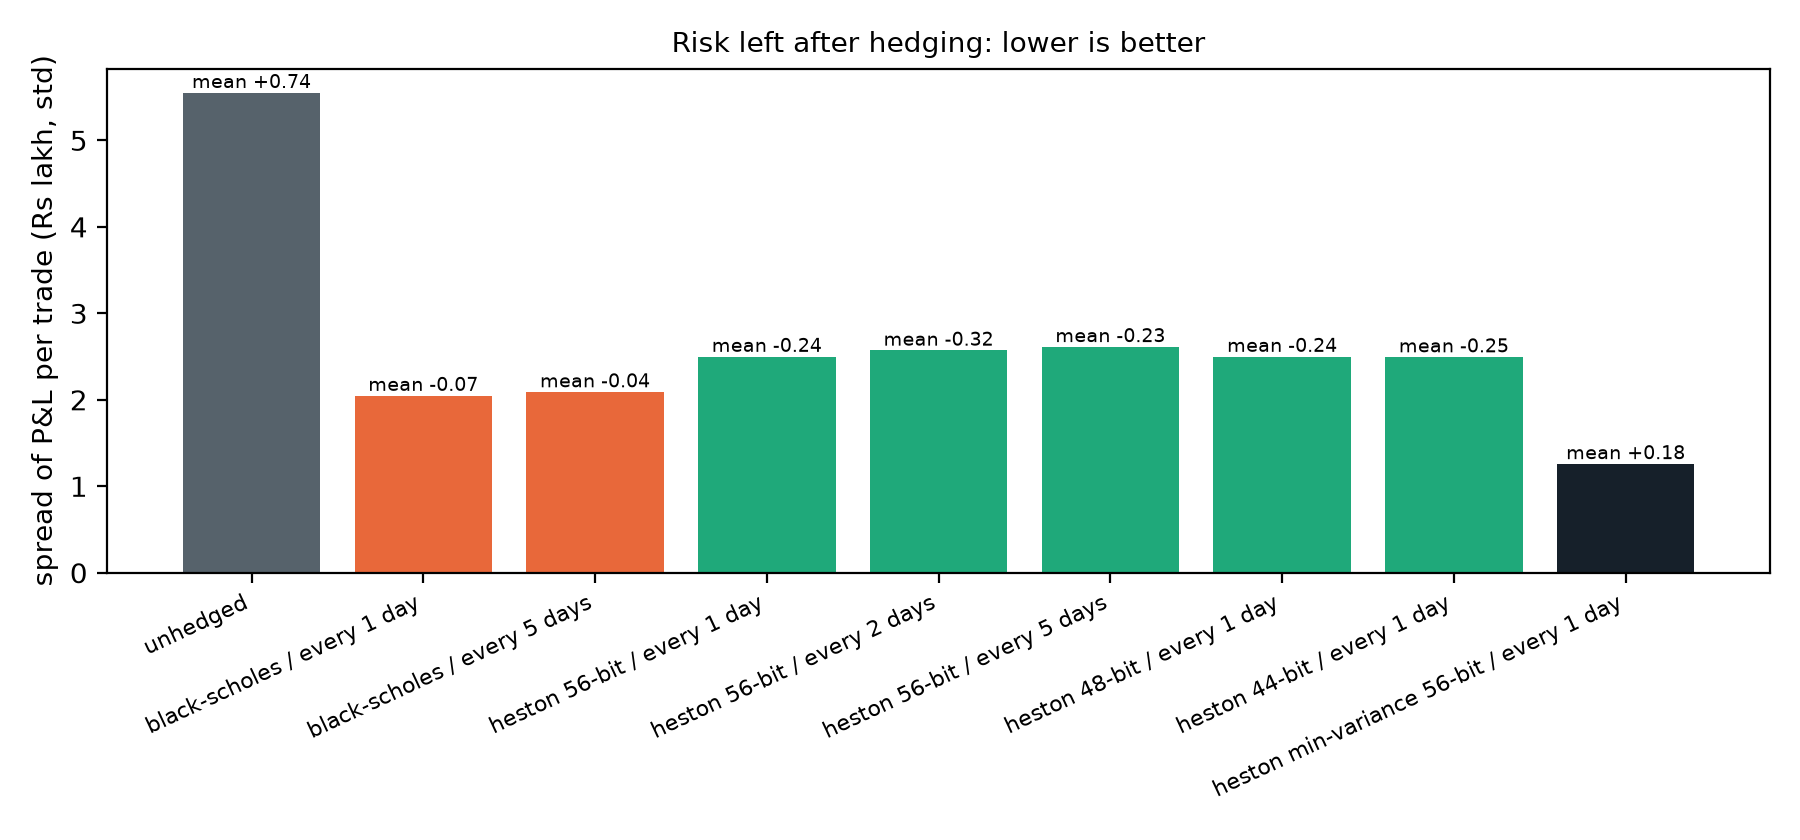
\includegraphics[width=\textwidth]{figures/fig12_hedge_risk.png}\\[4pt]
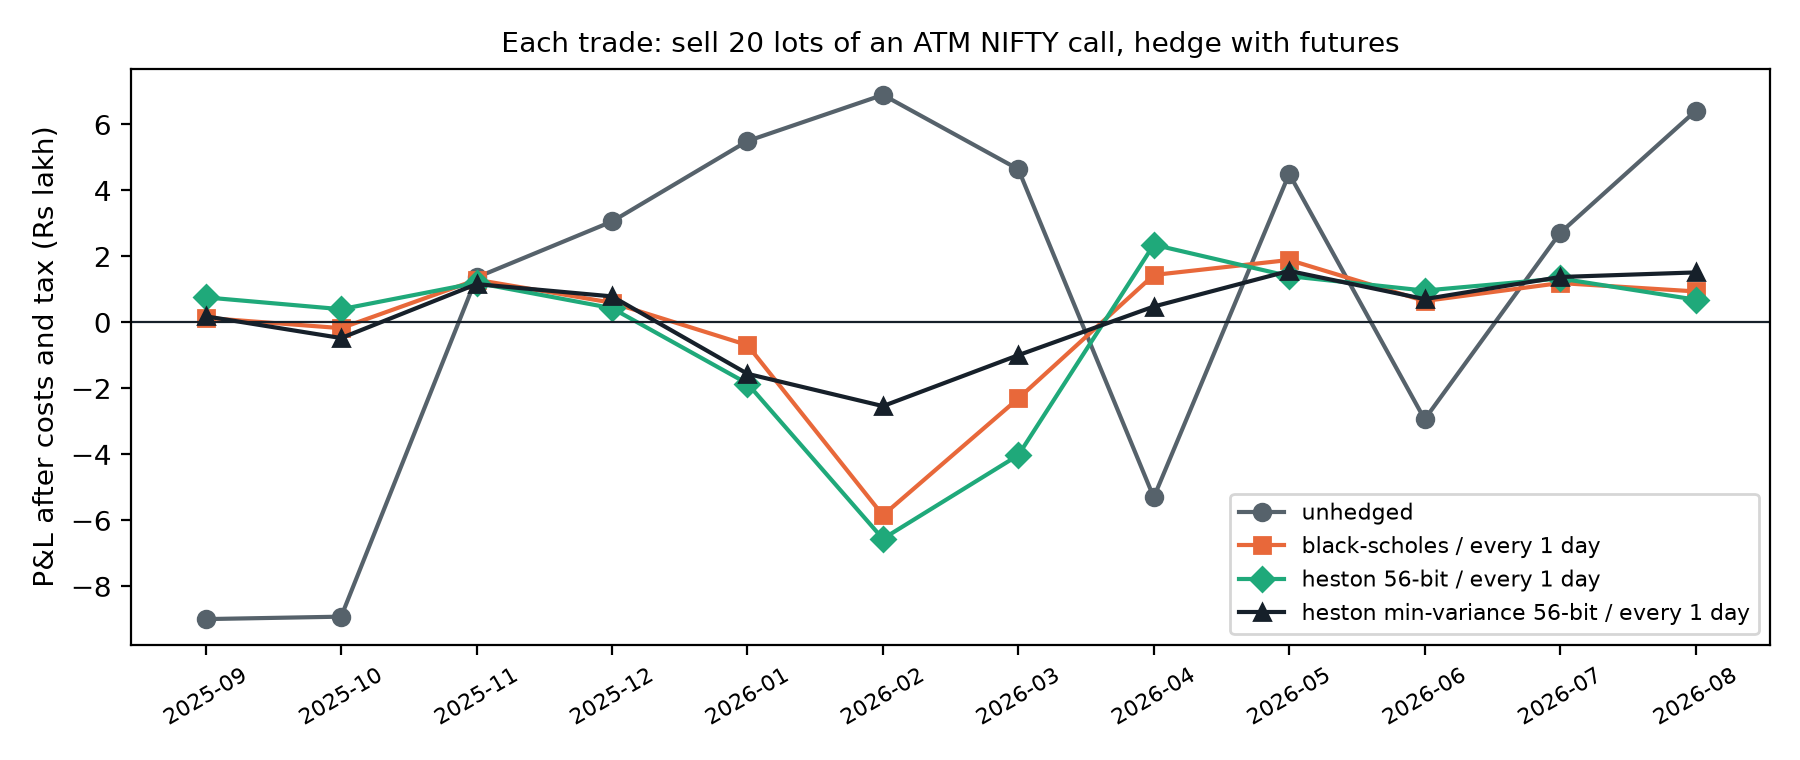
\includegraphics[width=\textwidth]{figures/fig13_hedge_pnl_per_trade.png}
\caption{Top: risk left after each hedge, including rebalancing every 2 or 5 days and
the 48- and 44-bit engines. Bottom: each trade's profit or loss.}
\end{figure}

The Heston delta on its own hedged worse than Black--Scholes. This is expected: it
holds variance fixed, while on the index variance rises when the price falls. Adding
the vega term corrects that and gave the lowest risk of all the hedges, 39\% below
Black--Scholes, with a worst loss of \rupee2.54\,L instead of \rupee5.85\,L. With 12
trades this is a case study, not a statistical result: the minimum-variance hedge lost
less on 5 of the 12 trades, much of the gain comes from the worst trade, and a bootstrap
gives about an 88\% chance that its risk is genuinely lower. Word length did not
matter: deltas from 48-bit and 44-bit engines differ from the 56-bit ones by at most
$1.7\times10^{-4}$ and $1.6\times10^{-3}$, below the resolution of whole futures lots;
the 48-bit hedge traded exactly the same lots as the 56-bit one.

\useful{The illustration shows a use for having all Greeks at once: the hedge that
worked best combines two Greeks of the same option, delta and variance vega, which the
engine produces together in one pass. Its benefit comes from the formula, not from the
hardware, and needs more trades before it can be claimed. It also shows that for
hedging, a 48-bit engine would be enough.}

\subsection{Improvement over the first generation}
\begin{table}[H]
\centering
\small
\begin{tabularx}{\textwidth}{@{}l Y Y@{}}
\toprule
& \textbf{First generation (hand-written)} & \textbf{Generated engine}\\
\midrule
Cycles, price + 9 Greeks & 433,779 & \textbf{4,733} (92$\times$ fewer)\\
Cost of the Greeks & 2.16 pricings & \textbf{1.04} pricings\\
Advantage over bump-and-reprice & 8.8$\times$ & \textbf{18.4$\times$}\\
Multipliers & 159 dedicated 64$\times$64 (over 1,000 DSP) & \textbf{8 shared} (72 DSP)\\
Dividers & 28 bit-serial per term, 80\% of latency & \textbf{none}\\
Terms & one after another & \textbf{16 overlapping}\\
Fits a Zynq-7020 & no & \textbf{yes}, 73\% LUT\\
Run on silicon & no & \textbf{yes}, bit-exact\\
Error bound & price and Greeks, $\le 0.21$ & price and Greeks, $\le 0.103$\\
\bottomrule
\end{tabularx}
\caption{The first-generation engine against the generated engine.}
\end{table}

\useful{Moving from a hand-written state machine to a generated, shared, pipelined
datapath is what made the design fast enough to matter and small enough to fit a
low-cost FPGA.}

% =====================================================================
\section{Timeline}
\label{sec:timeline}

The project started on 15 August 2026; the paper is to be complete by 29 October
2026. Work up to 1 October is done; the rest is the plan (Table~\ref{tab:timeline},
Figure~\ref{fig:gantt}).

\begin{table}[H]
\centering
\small
\begin{tabularx}{\textwidth}{@{}l Y l@{}}
\toprule
\textbf{Dates} & \textbf{Work} & \textbf{Status}\\
\midrule
15--20 Aug & Black-Scholes and Heston models, software adjoint engine, MATLAB and C++ prototypes & Done\\
21 Aug -- 9 Sep & First-generation hand-written FPGA engine and its validation & Done\\
10--17 Sep & Fixed-point precision fixes, error bound, bump-and-reprice baseline, the datapath generator; design fits a Zynq-7020 & Done\\
18--24 Sep & Vivado implementation flow; project documentation & Done\\
25--27 Sep & AXI4-Lite interface, ZedBoard designs, first complete route (79\,MHz) & Done\\
28--29 Sep & On silicon: one vector, then 50 cases bit-exact; put-call parity; literature check & Done\\
30 Sep -- 1 Oct & CPU comparison; results dashboard and report & Done\\
1 Oct & Hand-derived analytic and optimised bump CPU baselines; strike-chain design study (\S\ref{sec:chain}) & Done\\
\midrule
5--6 Oct & ZedBoard bitstream rebuilt with put-call parity and refitted ranges; 50-case sweep repeated, 450 / 450 bit-exact & Done\\
6 Oct & Forward-mode hardware baselines (\S\ref{sec:modes}); bound stated as first order and checked in 50-digit arithmetic; COS truncation error as a separate term (\S\ref{sec:methoderr}); held-out range sweep; claims corrected & Done\\
1--13 Oct & Hedging case study on real NIFTY data (first results, \S\ref{sec:hedging}); next: verify charges with a broker, more trades & In progress\\
1 Oct & Validation sweep over 10,500 inputs including hard regimes; latency accounting (host steps, configurations) & Done\\
1 Oct & Shift ranges refitted at the domain edges; all designs regenerated and re-verified & Done\\
6--8 Oct & CPU timings on an idle machine & Next\\
6--12 Oct & Power from simulated switching activity, a board power measurement, and CPU package power, for energy per Greek set on both sides & Planned\\

13--15 Oct & Freeze results; regenerate all figures and tables & Planned\\
13--22 Oct & Write the paper: introduction, related work, architecture, results & Planned\\
22--27 Oct & Review with the supervisor; revisions & Planned\\
26--28 Oct & Final literature re-check; proofreading & Planned\\
\hi 29 Oct & \textbf{Paper complete} & Target\\
After 29 Oct & Generator derives the reverse sweep automatically; a second pricing model & Next paper\\
\bottomrule
\end{tabularx}
\caption{Project timeline.}
\label{tab:timeline}
\end{table}

\begin{figure}[H]
\centering
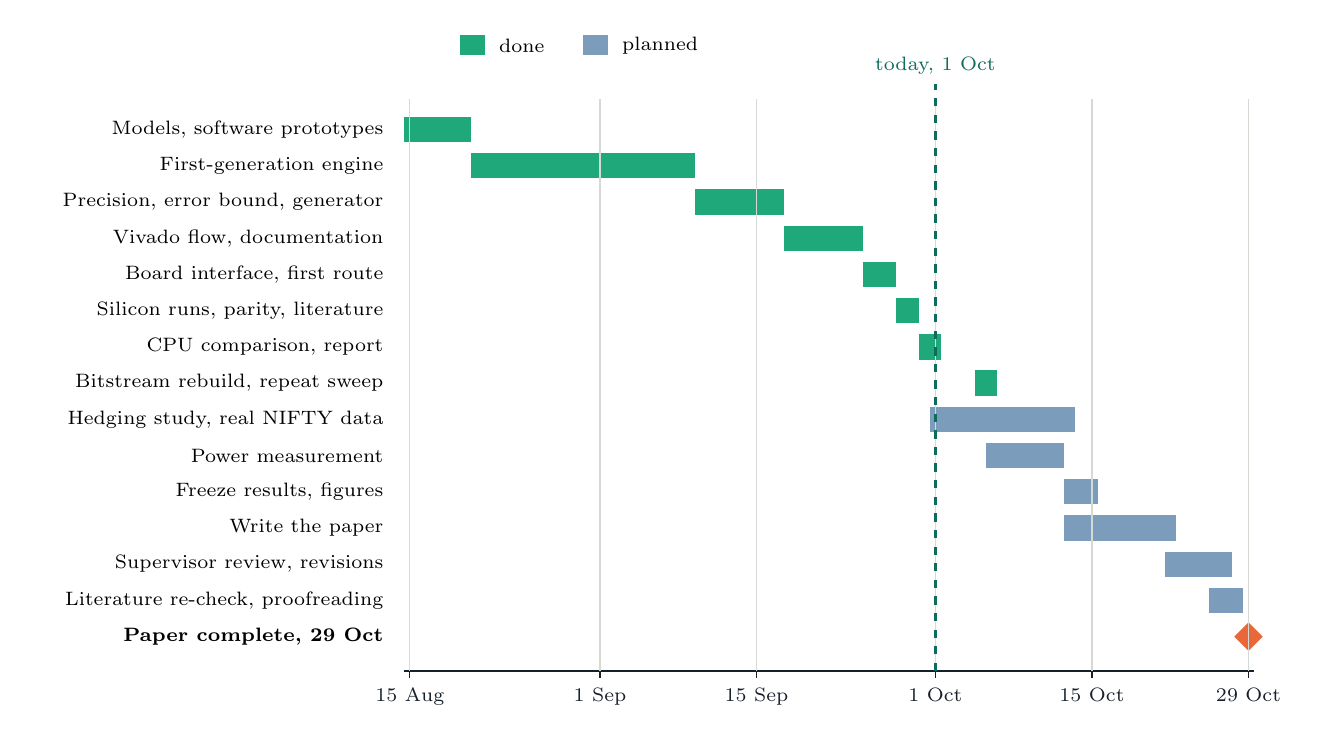
\begin{tikzpicture}[x=0.142cm, y=0.46cm]
  % day 0 = 15 Aug; 75 = 29 Oct
  \newcommand{\ganttbar}[5]{% row, label, start day, end day, colour
    \node[font=\scriptsize, anchor=east, text width=4.4cm, align=right] at (-1,-#1+0.35) {#2};
    \fill[#5] (#3,-#1) rectangle (#4+1,-#1+0.7);}
  \ganttbar{1}{Models, software prototypes}{0}{5}{aad}
  \ganttbar{2}{First-generation engine}{6}{25}{aad}
  \ganttbar{3}{Precision, error bound, generator}{26}{33}{aad}
  \ganttbar{4}{Vivado flow, documentation}{34}{40}{aad}
  \ganttbar{5}{Board interface, first route}{41}{43}{aad}
  \ganttbar{6}{Silicon runs, parity, literature}{44}{45}{aad}
  \ganttbar{7}{CPU comparison, report}{46}{47}{aad}
  \ganttbar{8}{Bitstream rebuild, repeat sweep}{51}{52}{aad}
  \ganttbar{9}{Hedging study, real NIFTY data}{47}{59}{plan}
  \ganttbar{10}{Power measurement}{52}{58}{plan}
  \ganttbar{11}{Freeze results, figures}{59}{61}{plan}
  \ganttbar{12}{Write the paper}{59}{68}{plan}
  \ganttbar{13}{Supervisor review, revisions}{68}{73}{plan}
  \ganttbar{14}{Literature re-check, proofreading}{72}{74}{plan}
  \node[diamond, fill=bump, inner sep=2.6pt] at (75.5,-15+0.35) {};
  \node[font=\scriptsize\bfseries, anchor=east, text width=4.4cm, align=right] at (-1,-15+0.35) {Paper complete, 29 Oct};
  \draw[ink] (0,-15.6) -- (76,-15.6);
  \foreach \d/\t in {0/15 Aug, 17/1 Sep, 31/15 Sep, 47/1 Oct, 61/15 Oct, 75/29 Oct} {
    \draw[ink] (\d+0.5,-15.6) -- ++(0,-0.2) node[below, font=\scriptsize] {\t};
    \draw[rulec] (\d+0.5,-15.6) -- (\d+0.5,0.2);
  }
  \draw[accent, thick, dashed] (47.5,-15.6) -- (47.5,0.6) node[above, font=\scriptsize, text=accent] {today, 1 Oct};
  \fill[aad] (5,1.4) rectangle ++(2.2,0.55); \node[font=\scriptsize, anchor=west] at (7.6,1.67) {done};
  \fill[plan] (16,1.4) rectangle ++(2.2,0.55); \node[font=\scriptsize, anchor=west] at (18.6,1.67) {planned};
\end{tikzpicture}
\caption{Timeline from project start to the paper deadline.}
\label{fig:gantt}
\end{figure}

% =====================================================================
\begin{thebibliography}{99}
\small
\bibitem{heston} S. L. Heston, ``A closed-form solution for options with stochastic
volatility with applications to bond and currency options,'' \emph{Review of Financial
Studies}, 6(2):327--343, 1993.
\bibitem{fang} F. Fang and C. W. Oosterlee, ``A novel pricing method for European
options based on Fourier-cosine series expansions,'' \emph{SIAM Journal on Scientific
Computing}, 31(2):826--848, 2008.
\bibitem{giles} M. Giles and P. Glasserman, ``Smoking adjoints: fast Monte Carlo
Greeks,'' \emph{Risk}, January 2006.
\bibitem{capriotti} L. Capriotti, ``Fast Greeks by algorithmic differentiation,''
\emph{Journal of Computational Finance}, 14(3):3--35, 2011.
\bibitem{savine} A. Savine, \emph{Modern Computational Finance: AAD and Parallel
Simulations}, Wiley, 2018.
\bibitem{aadreview} L. Capriotti and M. Giles, ``15 years of adjoint algorithmic
differentiation in finance,'' 2024.
\bibitem{klai1} M. Klaisoongnoen, N. Brown and O. T. Brown, ``Low-power option Greeks:
efficiency-driven market risk analysis using FPGAs,'' \emph{HEART}, 2022.
\bibitem{klai2} M. Klaisoongnoen et al., ``Fast and energy-efficient derivatives risk
analysis: streaming option Greeks on Xilinx and Intel FPGAs,'' \emph{H2RC}, 2022.
\bibitem{vitis} AMD (Xilinx), \emph{Vitis Quantitative Finance Library}, open-source
library, \url{https://github.com/Xilinx/Vitis_Libraries}.
\bibitem{survey} A. O Mahony, B. Hanzon and E. Popovici, ``The role of FPGAs in modern
option pricing techniques: a survey,'' \emph{Electronics}, 13(16):3186, 2024.
\bibitem{zhang} B. Zhang and C. W. Oosterlee, ``Option pricing with COS method on
graphics processing units,'' \emph{IEEE IPDPS Workshops}, 2009.
\bibitem{linnainmaa} S. Linnainmaa, ``Taylor expansion of the accumulated rounding
error,'' \emph{BIT Numerical Mathematics}, 16:146--160, 1976.
\bibitem{codipack} M. Sagebaum, T. Albring and N. R. Gauger, ``High-performance
derivative computations using CoDiPack,'' \emph{ACM Transactions on Mathematical
Software}, 45(4), 2019.
\bibitem{cui} Y. Cui, S. del Ba\~no Rollin and G. Germano, ``Full and fast calibration
of the Heston stochastic volatility model,'' \emph{European Journal of Operational
Research}, 263(2):625--638, 2017.
\end{thebibliography}

\end{document}
